\documentclass[a4paper,12pt]{book}
\usepackage{enumitem}
\usepackage{url}
\usepackage{hyperref}
\usepackage{amsmath}
\usepackage[catalan]{babel}
\usepackage{xcolor}
\usepackage{graphicx}
\usepackage{comment}
\usepackage{listings}
\usepackage{array}
\usepackage[utf8]{inputenc}
\usepackage[T1]{fontenc}
\usepackage{float}
\usepackage{amsfonts}
\usepackage[most]{tcolorbox}


\lstset{
    literate=  % Defineix com traduir caràcters especials
        {á}{{\'a}}1 {é}{{\'e}}1 {í}{{\'i}}1 {ó}{{\'o}}1 {ú}{{\'u}}1
        {Á}{{\'A}}1 {É}{{\'E}}1 {Í}{{\'I}}1 {Ó}{{\'O}}1 {Ú}{{\'U}}1
        {à}{{\`a}}1 {è}{{\`e}}1 {ì}{{\`i}}1 {ò}{{\`o}}1 {ù}{{\`u}}1
        {À}{{\`A}}1 {È}{{\'E}}1 {Ì}{{\`I}}1 {Ò}{{\`O}}1 {Ù}{{\`U}}1
        {ä}{{\"a}}1 {ë}{{\"e}}1 {ï}{{\"i}}1 {ö}{{\"o}}1 {ü}{{\"u}}1
        {Ä}{{\"A}}1 {Ë}{{\"E}}1 {Ï}{{\"I}}1 {Ö}{{\"O}}1 {Ü}{{\"U}}1
        {â}{{\^a}}1 {ê}{{\^e}}1 {î}{{\^i}}1 {ô}{{\^o}}1 {û}{{\^u}}1
        {Â}{{\^A}}1 {Ê}{{\^E}}1 {Î}{{\^I}}1 {Ô}{{\^O}}1 {Û}{{\^U}}1
        {ã}{{\~a}}1 {ẽ}{{\~e}}1 {ĩ}{{\~i}}1 {õ}{{\~o}}1 {ũ}{{\~u}}1
        {Ã}{{\~A}}1 {Ẽ}{{\~E}}1 {Ĩ}{{\~I}}1 {Õ}{{\~O}}1 {Ũ}{{\~U}}1
        {ç}{{\c c}}1 {Ç}{{\c C}}1
        {œ}{{\oe}}1 {Œ}{{\OE}}1 {æ}{{\ae}}1 {Æ}{{\AE}}1
        {ß}{{\ss}}1 {«}{{\guillemotleft}}1 {»}{{\guillemotright}}1
        {ñ}{{\~n}}1 {Ñ}{{\~N}}1 {¿}{{?`}}1 {¡}{{!`}}1,
    inputencoding=utf8,
    extendedchars=true,
    basicstyle=\ttfamily,
    breaklines=true,
    showstringspaces=false
}

% We're working with A4, which is 21cm by 29.7
\setlength{\paperwidth}{210mm}
\setlength{\paperheight}{297mm}
%\setlength{\hoffset}{-15mm}
\setlength{\voffset}{-25mm}
\setlength{\textheight}{242mm}
\setlength{\topmargin}{10mm}
\setlength{\headheight}{10mm}
\setlength{\headsep}{10mm}
\setlength{\footskip}{1.2cm} %def=30pt=1.054cm

\setlength{\textwidth}{155mm}
\setlength{\oddsidemargin}{5mm}
\setlength{\evensidemargin}{-5mm}

% Espai entre línies de 1.5
\renewcommand{\baselinestretch}{1.5}

\usepackage{fancyhdr}
\pagestyle{fancy}
\pagenumbering{arabic}
\setlength{\parindent}{0truecm}
\lhead{}
\chead{}
\rhead{}
\lfoot{}
\cfoot{}
\rfoot{}
\renewcommand{\headrulewidth}{0pt}



\makeindex

\usepackage{titlesec}

\titleformat{\chapter}[block]
  {\normalfont\huge\bfseries\center}{\thechapter.}{1em}{\Huge}
\titlespacing*{\chapter}{-0.5cm}{-1.5cm}{0.5cm}
\renewcommand{\chaptername}{}

\begin{document}



\newlength{\centeroffset}
\setlength{\centeroffset}{-0.5\oddsidemargin}
\addtolength{\centeroffset}{0.5\evensidemargin}
%\addtolength{\textwidth}{-\centeroffset}
\thispagestyle{empty}
\vspace*{\stretch{1}}
\noindent\hspace*{\centeroffset}\begin{minipage}{\textwidth}
% \begin{center}
%       \includegraphics[width=0.8\textwidth]{./../figures/matesLliure.pdf}
% \end{center}
\vspace*{3truecm}

\flushright
{\Huge\bfseries 
  Inteligencia Artificial TR
}
\noindent\rule[-1ex]{\textwidth}{5pt}\\[4.5ex]
\end{minipage}

\vspace{\stretch{1}}
\noindent\hspace*{\centeroffset}\begin{minipage}{\textwidth}
\flushright
{\bfseries 
	Jiajun Xia i Rui Chen
}
\end{minipage}
%\addtolength{\textwidth}{\centeroffset}
\vspace{\stretch{2}}


\pagebreak

\vspace*{16truecm}

	\begin{quote}
	\textbf{Avís legal}

	  Copyright \copyright{}  Nom.
	  Es garanteix permís per copiar, distribuir i modificar aquest document segons els termes de la GNU Free Documentation License, versió 1.3 o qualsevol posterior publicada per la Free Software Foundation. Es disposa d'una còpia d'aquesta llicència a~\href{http://www.fsf.org}{http://www.fsf.org} i a l'annex~\ref{a:license}.
	\end{quote}	





\endinput


\frontmatter

\cleardoublepage

% \newtcolorbox{modernquote}{
  colback=white,
  colframe=white,
  boxrule=0pt,
  leftrule=2pt,
  colbacktitle=white,
  coltitle=black,
  arc=0pt,
  outer arc=0pt,
  left=10pt,
  right=10pt,
  top=8pt,
  bottom=8pt,
  before skip=12pt,
  after skip=12pt,
  enhanced jigsaw,
  parbox=false,
  fontupper=\small
}
\setlength{\parskip}{4pt}
\begin{modernquote}
\textsc{\textbf{Agraïments}}\par
\setstretch{1.1}
\raggedright
Volem agrair al nostre professor de matemàtiques, \textbf{Fernando Garcia}, pel suport constant que ens ha portat durant la realització d’aquest treball, per la seva claredat en la resolució de dubtes i problemes, i sobretot per haver-se ofert voluntàriament a ser el nostre tutor. La seva ajuda diària, malgrat la gran càrrega de treball amb altres projectes de recerca. Ha estat fonamental per a nosaltres.\par

També volem expressar el nostre agraïment al professor de la universitat \textbf{...}, que ens ha facilitat diversos recursos relacionats amb la intel·ligència artificial, incloent-hi un curs d’iniciació molt valuós.\par

Donem les gràcies a \textbf{Jia Zheng}, un amic que ens ha ofert suport extern en la construcció de la nostra xarxa neuronal.\par

Finalment, volem agrair a \textbf{Eric Garcia}, company nostre, per haver-se ofert a revisar i examinar el nostre treball de recerca, així com a totes les persones que ens han donat suport al llarg del procés i han fet possible la realització d’aquest projecte.
\end{modernquote}
\clearpage


\cleardoublepage
\setcounter{tocdepth}{2}
\renewcommand\contentsname{Índex de continguts}
\tableofcontents
\label{i:tableofcontents}

\mainmatter
\pagestyle{fancy}
\fancyhf{}
\fancyhead[RE,LO]{Intel·ligència Artificial TR}
\fancyhead[LE,RO]{\leftmark}
\fancyfoot[RE,LO]{Institut Sants}
\fancyfoot[LE,RO]{\thepage}
\renewcommand{\headrulewidth}{2pt}
\renewcommand{\footrulewidth}{1pt}


\chapter{Answer}




\newtcolorbox{modernquote}{
    colback=gray!10,
    colframe=white,
    boxrule=0pt,
    leftrule=4pt,
    colupper=black,
    arc=0pt,
    outer arc=0pt,
    left=8pt,
    right=8pt,
    top=8pt,
    bottom=8pt,
    before skip=12pt,
    after skip=12pt,
    enhanced jigsaw,
    borderline west={4pt}{0pt}{gray!60}
}
\begin{modernquote}
    Dwar Ev va soldar cerimoniosament la connexió final amb or. Els ulls d’una dotzena de càmeres de televisió l’observaven i el subeter transmetia a tot l’univers una dotzena d’imatges del que ell feia.

Es va redreçar i va assentir amb el cap a Dwar Reyn, després es va col·locar al costat de l’interruptor que completaria el contacte quan el llancés. L’interruptor que connectaria, tot d’una, totes les monstruoses màquines de computació de tots els planetes habitats de l’univers —noranta-sis mil milions de planetes— en el supercircuit que les enllaçaria totes en una sola supercalculadora, una màquina cibernètica que combinaria tot el coneixement de totes les galàxies.

Dwar Reyn va parlar breument als bilions d’oients i espectadors. Després d’un moment de silenci, va dir:

—Ara, Dwar Ev.


Dwar Ev va activar l’interruptor. Hi va haver un brunzit poderós, l’alliberament d’energia procedent de noranta-sis mil milions de planetes. Les llums van centellejar i després es van apagar al llarg del tauler de quilòmetres de llargada.

Dwar Ev es va fer enrere i va respirar profundament.

—L’honor de fer la primera pregunta és teu, Dwar Reyn.



—Gràcies —va dir Dwar Reyn—. Serà una pregunta que cap màquina cibernètica per si sola no ha estat capaç de respondre.


Es va girar per mirar la màquina.

—Hi ha un Déu?


La veu poderosa va respondre sense vacil·lar, sense que fes clic cap relé:

—Sí, ara hi ha un Déu.


Una por sobtada va aparèixer al rostre de Dwar Ev. Va saltar per agafar l’interruptor.

Un llamp, vingut d’un cel sense núvols, el va fulminar i va fondre l’interruptor tancat.


    \hfill \textit{Brown, Fredric. "Answer." Angels and Spaceships, E. P. Dutton \& Co., 1954.}
\end{modernquote}



\chapter{Introducció}
\label{c:intro}

Cita bibliogràfica: \cite{TP} bla bla bla
\section {Prova}
Aquest es la practica que he fet en Latex.Un section.
\section{Equació}
Aquí faig una equació $$ E = mc^2 $$

\section{Coses importants}
\begin{enumerate}
  \item Primer Element
  \item Segon Element
  \item Tercer Element
\end{enumerate}

\date{\today}


\begin{align}
  \text{He fet un align} \\
\end{align}

\begin{tabular}{|c|c|}
 \hline
 jo & ella \\
 \hline
 ell & jo \\
 \hline
\end{tabular}





\chapter{Objectius}
\label{c:objectius}
Tal com podem veure en la \nameref{c:intro}, el nostre objectiu del TR (Treball de Recerca) és construir una xarxa neuronal, però no ens val qualsevol xarxa neuronal, ja que n'hi han d'infinites  models, per dur a terme aquest estudi, vam seleccionar tres models de xarxes neuronals diferents: una implementada en Python, una altra basada en fulls de càlcul i una tercera aplicada a un exemple real del joc Mobile Legends: Bang Bang. A partir d'aquí desglossem 4 apartats amb diferents objectius: \nameref{sec:Xarxa neuronal amb llenguatge de programació} \nameref{sec:Xarxa neuronal amb fulls de calculs} \nameref{sec:Xarxa neuronal amb un cas real} \nameref{sec:Objectius personals}


\section{Xarxa neuronal amb llenguatge de programació}\label{sec:Xarxa neuronal amb llenguatge de programació}
En aquest apartat fixem els objectius, o més ben dit requisits de la xarxa neuronal que farem amb llenguatge de programació.
\begin{enumerate}[label=\alph*)]
 \item Fer ús de Python com a llenguatge principal
 \item Utilitzar llibreries bàsiques com \texttt{NumPy} i \texttt{TensorFlow} per facilitar els càlculs
 \item Crear una xarxa capaç de reconèixer patrons senzills (per exemple, classificació de dades)
 \item Documentar el procés de disseny i d’implementació del codi
\end{enumerate}


\section{Xarxa neuronal amb fulls de calculs}\label{sec:Xarxa neuronal amb fulls de calculs}
Els objectius d’aquest apartat són:
\begin{enumerate}[label=\alph*)]
\item Implementar manualment els càlculs bàsics d’una xarxa neuronal en un full de càlcul (propagació cap endavant i retropropagació)
\item Mostrar de forma visual com funcionen les operacions matemàtiques internes
\item Comparar l’eficiència i la dificultat respecte a la implementació en Python
\end{enumerate}


\section{Xarxa neuronal amb un cas real}\label{sec:Xarxa neuronal amb un cas real}
Aquí volem aplicar els coneixements anteriors a un context més proper i pràctic:
\begin{enumerate}[label=\alph*)]
\item Escollir un cas concret relacionat amb el joc \textit{Mobile Legends: Bang Bang}
\item Recrear el cas real e intentar apropar-nos al màxim a la seva lògica
\item Comunicar-nos amb els treballadors del joc com a font de recursos
\end{enumerate}


\section{Objectius personals}\label{sec:Objectius personals}
A més dels objectius tècnics, també hi ha objectius d’aprenentatge personal:
\begin{enumerate}[label=\alph*)]
\item Dominar les funcionalitats basiques del \LaTeX, Vim, Github i Git
\item Millorar el nostre forma de redactar
\item enriquir de coneixements i gaudir del treball
\end{enumerate}





%
%
\chapter{Recerca prèvia}
\label{c:recerca prèvia}
\section{La Història de la IA: Des dels orígens fins avui}
\begin{enumerate}
     \item \textbf{El Naixement d'una Idea Revolucionària (1956)}

             Alan Turing, el geni matemàtic que va desxifrar Enigma, una màquina emprada pels nazis per codificar els seus missatges durant la Segona Guerra Mundial (1939-1945), va fer una pregunta provocadora a la comunitat científica: "Podran les màquines pensar alguna vegada?". Aquesta qüestió va obrir les portes a un nou camp d’estudi. En 1956 John McCarthy, Marvin Minsky i d'altres especialistes van nominar oficialment el terme ``intel·ligència artificial'' durant la conferència de Dartmouth, marcant l'inici d'una nova era tecnològica.

      \item \textbf{El Joc que ho va canviar tot: The Imitation Game/El test de Turing}

            L'origen de la IA es basa en un experiment molt senzill, però profund: El joc d'imitació (The imitation game), proposat per Alan Turing. Per respondre a la pregunta "Podran les màquines pensar alguna vegada?", Turing va dissenyar un joc que funcionava com a test per les màquines anomenat ``The Imitation Game''. Aquest test consistia a fer que un avaluador havia d'intercanviar textos escrits amb una persona i una màquina durant 5 minuts, aquest avaluador no sabia qui era qui i havia d'esbrinar qui era l'humà. Si la màquina aconseguia enganyar a l'avaluador passava el test i es considerava que la màquina havia aconseguit un nivell de comportament lingüístic equivalent al d'un humà, per tant, podríem considerar que les màquines poden pensar. Aquest joc ha estat evolucionant gràcies als avenços de la ciència i de la tècnica, i encara avui dia és conegut com el test de Turing.

     \item Les grans fites de la IA
        \subsubsection{1997: La màquina que va vèncer un campió}
            La supercomputadora Deep Blue desenvolupada per IBM va derrotar el campió mundial d’escacs, Garri Kaspàrov, demostrant que la IA podia superar els humans en jocs d’estratègia complexos.
        \subsubsection{2022: L'explosió de la IA}
         Milions d’usuaris van descobrir models com ChatGPT que podien escriure, traduir i programar amb un llenguatge gairebé humà, obrint nous horitzons en la interacció home-màquina.
        \subsubsection{2025: La IA en tots els àmbits}
        2025: La IA en Tots els Àmbits
        Avui, la IA està present en dibuix, contingut audiovisual, cotxes autònoms, medicina i molt més, amb models cada vegada més especialitzats i avançats.

\end{enumerate}

(Fonts:~\cite{McCarthy_Minsky_Rochester_Shannon_2006},~\cite{deepblue},
~\cite{chatGPT2022} i~\cite{10.1093/mind/LIX.236.433})


\section{Que és la IA?}
% Hem estat parlant molt durant aquest treball sobre la IA, i ara que em après quina és la seva història, hem de saber que és. \\
% Doncs bé, p
Podem definir la IA com sistemes de software i de hardware dissenyats per humans que actuen en la dimensió física o digital, és a dir, raonar sobre el coneixement, processant la informació derivada de dades i prendre les millors decisions per assolir l'objectiu donat. O dit d'un altra manera, és un camp de la informàtica que consisteix en un conjunt de capacitats intel·lectuats i cognitives expressades per un sistema informàtic creat pels humans, que té com a propòsit imitar la intel·ligència humana. \\

Un exemple d'IA i que tot el món coneix i utilitza és el ChatGPT, un xatbot impulsat per un model d'intel·ligència artificial generativa de l'empresa OpenAI. Fa servir tècniques de processament de llenguatge natural per comprendre preguntes fetes per l'usuari i generar respostes coherents en converses, simulant una interacció similar a la d'un humà. També pot generar o editar imatges, processar àudios, llegir arxius i molt més.

\section{Com funciona la IA?}
Una vegada que ja sabem que és una IA, ens toca entendre com funciona.
Les intel·ligències artificials utilitzen algoritmes i models matemàtics per processar grans quantitats de dades
i prendre accions basades en patrons i regles establertes a través de l'aprenentatge automàtic o l'aprenentatge profund.
Per tant, per funcionar necessitarà:

\begin{enumerate}
    \item \textbf{Dades}\\
    Les dades són fonamentals per la IA, ja que és la base de l'aprenentatge del model, per poder raonar, prendre decisions, i millorar la precisió. Aquí esdevenen uns exemples que pot haver-hi:
         \begin{itemize}
            \item \textbf{Base d'aprenentage}\\
            Els algoritmes de la IA necessiten a base de dades i una gran diversitat de dades per poder identificar patrons i construir prediccions.

           \item \textbf{Qualitat vs Quantitat}\\
            Una gran quantitat de dades ajudaran la IA a obtenir major precisió, però la qualitat és encara més important per la complexitat de dades que aporta, això evitarà que la IA cometes errors per informació incompleta.\textbf{ Per exemple:} En l'àmbit mèdic si vols que la IA faci una predicció i tan sols li dones una quantitat important de persones sanes i no d'altres exemplars, la IA simplement descartarà d'altres possibilitats que podrien haver-hi i només agafar la sana.

            \item \textbf{Exemples Reals}\\
            Els sistemes dels cotxes o assistents virtuals necessiten dades en temps reals per adaptar-se de l'entorn, també plataformes com Netflix o Spotify necessiten dades personalitzades per poder generar recomanacions amb precisió.
          \end{itemize}

    \item \textbf{Algorismes}\\
  Totes les aplicacions de la IA tenen el propòsit de capacitar la màquina perquè puguin operar com un humà. Tot això està basat en combinacions de diferents tipus d’algorismes. A continuació, explicarem els diferents tipus d’algorismes d’aprenentatge.
        \begin{itemize}
           \item \textbf{L'aprenentage automàtic(Machine learning)}\label{Aprenentatge_automàtic}
            És una branca crucial de la intel·ligència artificial, consisteix a cobrar vida a la màquina, donar-li el poder d'aprendre com els humans, executar tasques de manera autònoma i finalment, les infinites possibilitats d'evolucionar a través de l'experiència i molt més. Segons la UC Berkeley~\cite{Berkeley} el procés de l'aprenentatge automàtic és

            {\color{gray}
            \item \textbf{Mecanisme de predicció}
            \subitem\hspace*{-1\leftmargin} Un conjunt de regles o operacions matemàtics que analitza   les dades d'entrada i intenta identificar els patrons que busca el model.
            \item \textbf{Algoritme d'optimització}
            \subitem\hspace*{-1\leftmargin} El procés que ajusta automàticament el model per minimitzar l'error, modificant els paràmetres interns per millorar les prediccions futures.}
        \end{itemize}

             Segons Nvidia~\cite{Nvidia}, hi ha molts tipus d'aprenentatge automàtics:
            \begin{enumerate}
                \item \textbf{Aprenentatge supervisat}
                 L'aprenentatge supervisat és un tipus d'aprenentatge automàtic que treballa amb dades etiquetades, és a dir, dades que ja inclouen la solució o resultat desitjat. En aquest mètode, la intel·ligència artificial aprèn a associar les dades d'entrada amb les seves etiquetes corresponents, mitjançant l'anàlisi d'exemples prèviament resolts. Això li permet desenvolupar la capacitat de resoldre problemes nous aplicant la lògica i els patrons identificats a partir de dades reals.
                 \begin{comment}
                \textbf{Avantatges i desavanantatge:}
                 Aquest mètode destaca per la seva alta precisió en problemes ben definits, ja que al treballar   amb dades prèviament etiquetades pot assolir bons resultats en tasques de classificació i regressió. Una altra avantatge important és la facilitat per avaluar el rendiment dels models. A més, es tracta d'una àmplia àrea d'estudi amb una gran varietat d'algoritmes ben desenvolupats i optimitzats, com ara els arbres de decisió, els random forests, les màquines de vectors de suport (SVM) o les xarxes neuronals. Finalment, un cop entrenat adequadament, el model pot generalitzar el seu aprenentatge i fer prediccions útils sobre dades noves.\\

                 No obstant això, aquest enfocament també presenta alguns inconvenients significatius. El principal desavantatge és la seva forta dependència de conjunts de dades etiquetades, que sovint són costosos d'obtenir i preparar com las de medicines. Un altre problema freqüent és el sobreajustament (overfitting), que ocorre quan el model memoritza les dades d'entrenament en lloc d'aprendre patrons generals, la qual cosa provoca una perdua de raonament logica. Finalment, aquest mètode pot tenir dificultats per manejar certs tipus de dades no estructurades o problemes complexos, que podrien requerir quantitats molt grans de dades etiquetades per assolir un bon rendiment.
                 \end{comment}

                 \item \textbf{Aprenentatge semisupervisat}

                  L'aprenentatge semisupervisat representa un punt intermedi entre l'aprenentatge supervisat i el no supervisat, aprofitant tant dades etiquetades com no etiquetades per millorar l'eficiència dels models d'aprenentatge automàtic. Això funciona quan l'obtenció de les dades etiquetades són molt costoses i l'extracció de les característiques són molt complexes.

                  \item \textbf{Aprenentatge no supervisat}

                   L'aprenentatge no supervisat és una branca de l'aprenentatge automàtic que s'utilitza quan no es disposa de dades etiquetades. A diferència de l'aprenentatge supervisat, on el model rep exemples amb les seves solucions correctes, en aquest cas l'algorisme ha de descobrir per si mateix l'estructura i els patrons, fent un diagnòstic agrupant les característiques similars que poden haver-hi entre les dades.
                  Depenen dels tipus de problemes, les dades s'organitzen de diferents maneres.
                  \begin{itemize}
                   \item \textbf{Clustering:} Tècnica que agrupa les dades en funció de les seves similituds.
                   \item \textbf{Anomaly detection:} Cerca patrons que no encaixen amb el comportament normal.
                  \item \textbf{Association:} Cerca relacions i correlacions entre variables en grans conjunts de dades.
                   \item \textbf{Autocodificador:} Els autocodificadors són un tipus de xarxa neuronal artificial que aprèn a comprimir i reconstruir dades.
                 \end{itemize}
                  \item \hypertarget{Aprenentatge per reforç}{\textbf{Aprenentatge per reforç}}
                  L'aprenentatge per reforç és una altra branca de l'aprenentatge automàtic inspirada en la manera com els éssers vius aprenen mitjançant la interacció amb el seu entorn.
                 \begin{comment}
                 Com per exemple quan començem a jugar un videojoc, en els jocs rebem senyals de reforços, de si completem un nivell ens ortoga un trofeu, de si matem certs enemics guanyem bonificacions. Amb aquest sistema de penalitzacio i recompenses guia al jugador a millorar les seves tecniques de videojocs, i això  el podem aplicar perfectament en la IA.
                 \end{comment}


        %Totes les aprenantatges de reforç segueixen pragmaticament aquest esquema per l'aprenentage:

       %\begin{enumerate}
       %\item \textbf{Acció}
        %\item \textbf{Observació}
        %\item \textbf{Recompensa}
         %\item \textbf{Ajust d'estrategia}
        %\end{enumerate}

                  \item \textbf{Aprenentatge profund}
                   L'aprenentatge profund és una branca de l'aprenentatge automàtic que utilitza una xarxa neuronal amb múltiples capes per processar dades complexes i extreure'n característiques rellevants. Aquesta és inspirat en el funcionament del cervell humà, aquest enfocament permet identificar patrons i analitzar dades d'alta complexitat. Durant la fase d'identificació, s'empra un aprenentatge jeràrquic, és a dir, progressa gradualment des de característiques simples fins a patrons complexes.

     \begin{figure}[h!]
    \centering
    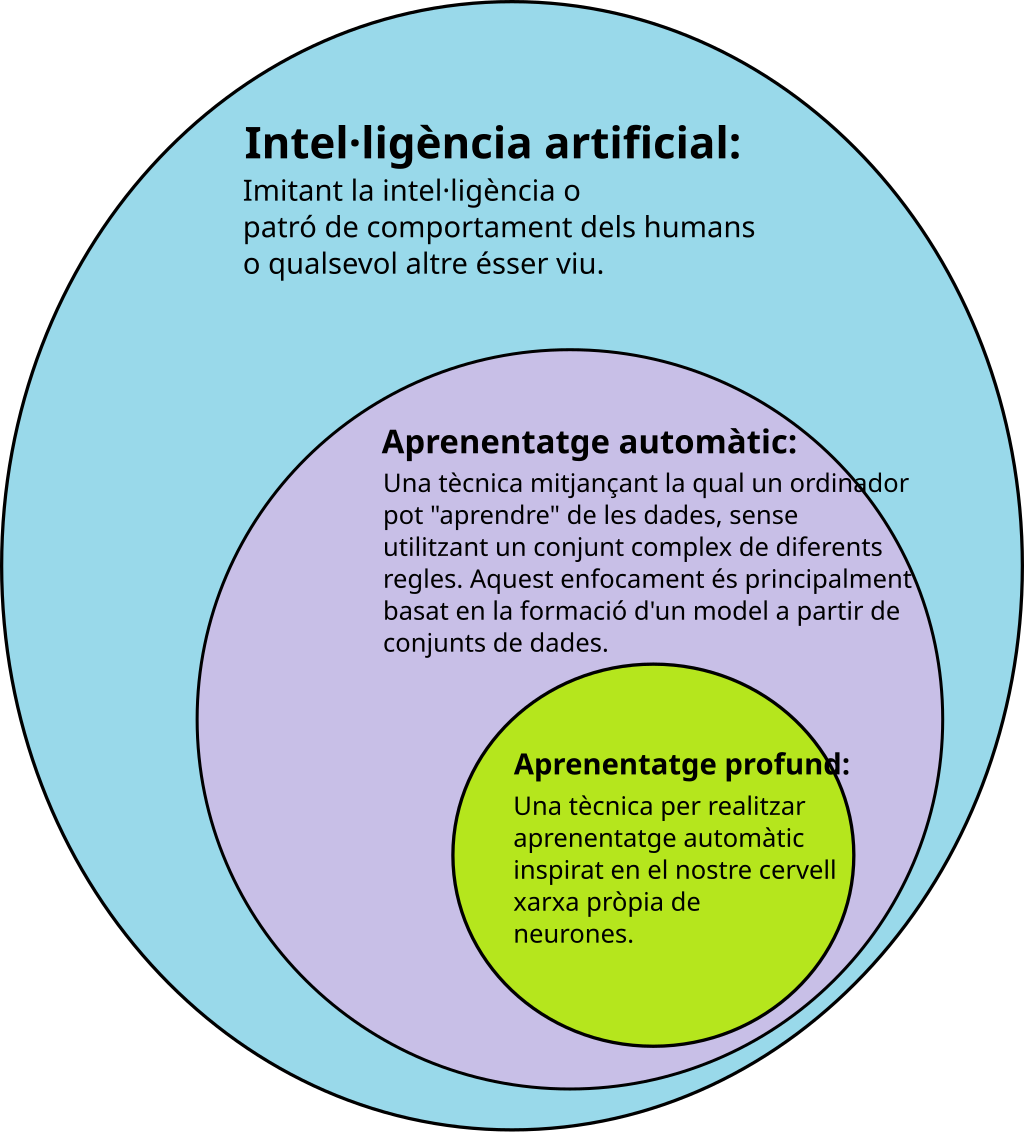
\includegraphics[width=0.2\textwidth]{./figures/Aprenentatge.png}
    \caption{Les capes que te la IA per funcionar}
    \end{figure}
          \end{enumerate}

  \item \textbf{Frameworks}
      Segons INESDI~\cite{INESDI}:\\
      {\color{gray}``Un Frameworks és, en el camp de la informàtica, una estructura conceptual que proporciona un conjunt d'eines, biblioteques i patrons de disseny per facilitar el desenvolupament de programari.
      %En altres paraules, són marcs de treball que funcionen com un esquelet predefinit, i sobre els quals es pot construir una aplicació o programari.

     Pel que fa als seus components, inclouen biblioteques de codi reutilitzables, mòduls predefinits, regles d'arxiu i directori, patrons de disseny i convencions de codificació.''}\\

      %Un Framework, en diferencia, de la biblioteca per el control total que pot tenir el usuari en tema estructura, i organitzacio dels codis, en canvi, una biblioteca està en mans del desenvolupador i només tens accés en els codis que et convenin de la biblioteca. Malgrat la utilitat que propociona no satisfeix la IA de la actualitat i han hagut de desarollar uns Frameworks especifics per la IA, de tal manera en que facilita el desarollament i l'entrenament dels models de la IA.

     \item \textbf{Ètica i Regulació}\\
      Un cop enteses totes les funcionalitats i capacitats de la intel·ligència artificial (IA), és fonamental aplicar-hi principis d’ètica i moral. Encara que la IA no sigui un ésser viu, és una eina creada per els  humans, i per tant cal establir-hi limitacions per evitar-ne els mals usos i garantir el respecte als drets humans i a la privacitat. Aquesta part és crucial en el desenvolupament d’una IA responsable. En aquest sentit, molts estats i organismes ja han publicat diverses lleis legítimes i regulacions. Algunes de les més rellevants són:
     \begin{itemize}
        \item \textbf{Llei d’IA de la Unió Europea (AI Act):} És la primera regulació integral sobre la IA. Classifica els sistemes d’IA segons el seu nivell de risc (inacceptable, alt, limitat i mínim) i estableix requisits estrictes per als usos d’alt risc, com la transparència, supervisió humana i seguretat.
           \item \textbf{Reglament General de Protecció de Dades (GDPR):} Tot i no ser exclusiu per a la IA, aquest reglament europeu protegeix la privacitat i les dades personals dels ciutadans. És clau en el desenvolupament d’IA que utilitza dades personals.
          \item \textbf{Principis ètics de la UNESCO sobre la IA (2021): Proposen una base global per al desenvolupament ètic de la IA, centrant-se en el respecte pels drets humans, la igualtat, la sostenibilitat, la no discriminació i la supervisió humana.}
          \item \textbf{Guies de l’OCDE sobre la IA:}Recomanen que els sistemes d’IA siguin transparents, responsables, segurs i que promoguin el benestar de la societat, ajudant a establir marcs internacionals de bones pràctiques.
     \end{itemize}


 \end{enumerate}





Fonts:~\cite{Universitat_oberta_catalunya},~\cite{Generalitat},~\cite{IBM_machine_learning},~\cite{Ultralytics},~\cite{bengio2012},~\cite{Ai_Act}, \cite{Algorismes} i ~\cite{Unesco}.

\section{Que és una xarxa neuronal artificial/biologica?}\label{sec:xarxa neuronal}
Una xarxa neuronal artificial és un model computacional inspirat en el funcionament del cervell humà, utilitzat en el camp de la intel·ligència artificial (IA) i l'aprenentatge automàtic (machine learning). Està dissenyada per reconèixer patrons, prendre decisions i aprendre a partir de dades, sense ser programada explícitament per a cada tasca específica.\\ \\
Si tenim una artificial també tindrem una biològica. Una xarxa neuronal biològica es refereix al sistema interconnectat de neurones (cèl·lules nervioses) en el cervell i el sistema nerviós dels éssers vius. Aquestes xarxes són la base de la cognició, l'aprenentatge i les funcions biològiques en humans i animals.\\


\section{Estructura d'una xarxa neuronal}\label{sec:3.6}
Una xarxa neuronal combina diverses capes de processament i utilitza elements simples que operen en paral·lel, simulen i estan inspirades en els sistemes nerviosos biològics com hem explicat en l'apartat \ref{sec:xarxa neuronal}. Consta d'una capa d'entrada, seguit d'una o diverses capes ocultes i finalment una capa de sortida. Les capes estan interconnectades mitjançant nodes o neurones; cada capa utilitza la sortida de la capa anterior com a entrada.

\begin{itemize}
 \item \textbf{Capa d'entrada:}La capa d'entrada és la primera capa que rep directament la informació d'entrada que es processarà.
 \item \textbf{Capes ocultes:}Les capes ocultes són les capes que estan entre la capa d'entrada i la de sortida, aquestes capes contenen unitats no observables. La seva funció principal és processar les dades de la capa d'entrada per extraure característiques i patrons complexos.  La quantitat de neurones que hi ha en les capes ocultes és un factor determinant per la capacitat que tingui la xarxa per capturar dades complexes.
 \item \textbf{Capa de sortida:}La capa de sortida és l'última capa que forma una xarxa neuronal i és l'encarregada de produir la predicció o el resultat final del model. Aquesta capa utilitza la informació que ha processat la o les capes ocultes i la transforma a través d'una funció activa per generar una sortida, que pot ser una predicció numèrica, una classificació o qualsevol altre resultat. Les neurones d'aquesta capa estan connectades amb totes les neurones de la capa anterior.
 \end{itemize}


\begin{figure}[h!]
    \centering
    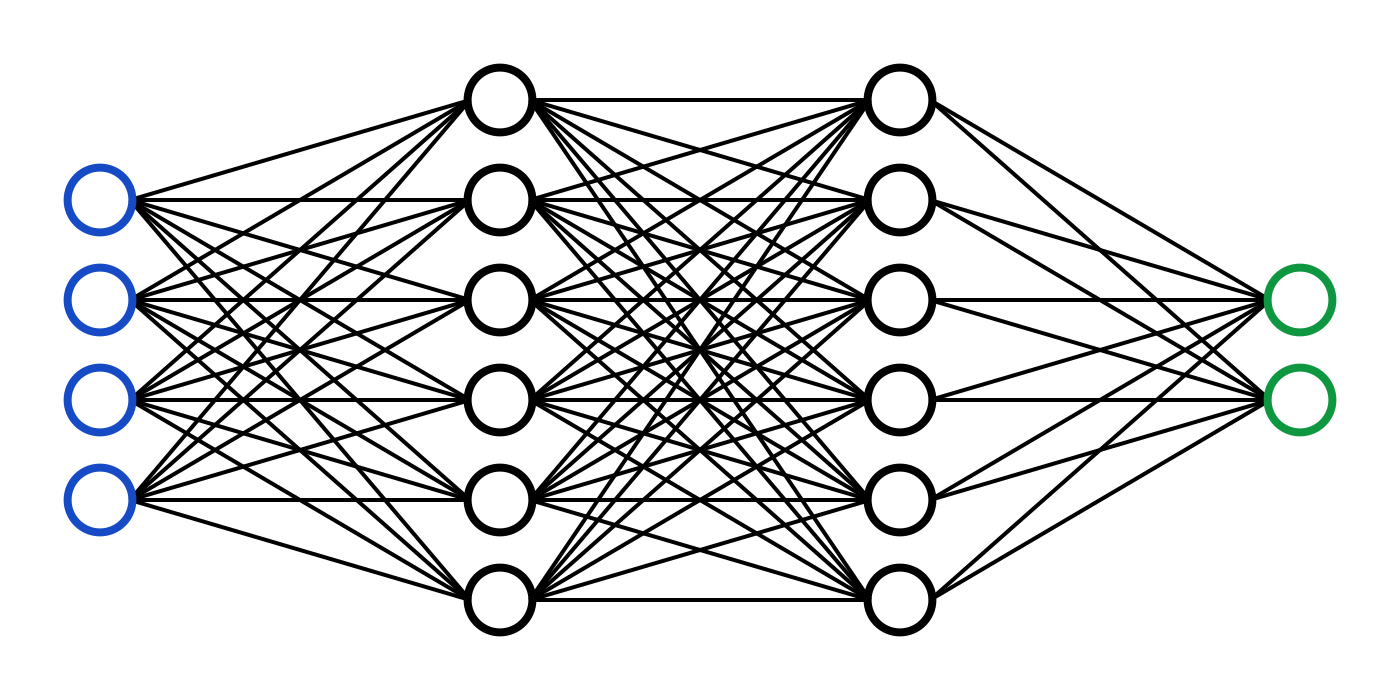
\includegraphics[width=0.5\textwidth]{./figures/xarxa.png}
    \caption{Estructura d'una xarxa neuronal}
\end{figure}

Fonts:~\cite{Hidden_layer} i~\cite{linkedin}

\section{Exemples de xarxes neuronals}
Hi ha molts tipus de xarxes neuronals, però com que el treball té una limitació de pàgines farem un resum de les xarxes més rellevants.

\begin{enumerate}
    \item \textbf{Perceptron (1958)}

    La primera xarxa neuronal, el Perceptró, va ser creada en la dècada de 1950 a 1960 pel psicòleg i informàtic Frank Rosenberg. Aquesta màquina permet prendre decisions binàries, per exemple respondre sí o no, de manera autònoma. \\
%     Aquest model pren varies entrades binaries $x_1$, $x_2$, fins les que calguin, i produeix una sola sortida binaria. Per calcular la sortida, Rosenblatt va introduir els ``pesos'', que está explicat a l'apartat \ref{sec:3.8}, els seus principals usos són decsions binàries senziles, o per crear funcions lògiques com OR o AND.
%%%%%%%%%%%%%% Això ho heu de simplificar molt, no cal entrar en tants detalls, feu com jo he fet a l'apartat anterior
    \item \textbf{Multiplayer Perceptron}
    El multiplayer perceptron és una ampliació de la percepció d'una única neurona a més d'una. A més, apareix el concepte de capes d'entrades, capes ocultes i capes de sortida, però amb valors d'entrada i sortida binàries.\\
    \item \textbf{Neurones sigmoide}
    Per aconseguir que les xarxes neuronals aprenguin per elles mateixes, és a dir, aprenentatge automàtic \ref{Aprenentatge_automàtic}, va ser necessari introduir un nou tipus de neurones, que són les Neurones Sigmoides, que són similars al perceptró, aquestes neurones en comptes de què les entrades siguin 1 o 0, puguin tenir valors com 0.5, o 0.374 o qualsevol altre valor real.\\

    %Ara les sorides en lloc de ser 0 o 1, serà d(w . x + b), on d serà la funció sigmoide, explicat en l'apartat \ref{sigmoide}. Aquesta va ser la primera funció d'activació \ref{Activació}.

    \item \textbf{Xarxa neuronal prealmentada (Feedforward)}
    Les xarxes neuronals prealimentades són les que les sortides d'una sola capa són utilitzades com entrades en la pròxima.
\end{enumerate}

\section{
Funció d'activació}\label{Activació}
Les funcions d'activació són un component integral de les xarxes neuronals que els permeten aprendre patrons complexos en les dades. Transformen el senyal d'entrada d'una neurona en un senyal de sortida que passa a la capa següent. Sense funcions d'activació, les xarxes neuronals es limitarien a modelar únicament relacions lineals entre entrades i sortides, és a dir, introdueixen la no-linealitat i produeixen la sortida de la neurona.

\begin{enumerate}
 \item \label{sigmoide}{\textbf{Funció sigmoide}}\\
 Una funció d'activació molt coneguda és la funció sigmoide. La seva fórmula és:
$$[ \sigma(x) = \frac{1}{1 + e^{-x}} ]$$

Aquesta funció matemàtica transforma qualsevol valor d'entrada real en un valor que està 0 i 1. La seva forma característica és una corba en forma de ``S''. Si el valor de $x$ que introduïm a la funció és molt gran o fins infinit $(\infty)$, llavors\ $\sigma$ serà 1; en canvi, si és molt petit o menys infinit $(-\infty)$,\ $\sigma$ serà 0, i si x = 0,  $\sigma$  serà 0,5.

\begin{figure}[h!]
    \centering
    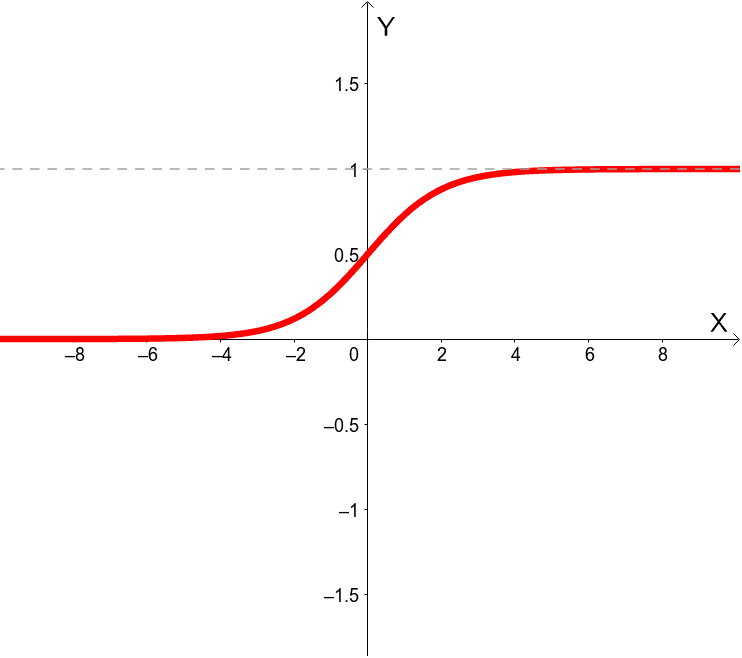
\includegraphics[width=0.5\textwidth]{./figures/grafica_sigmoide.png}
    \caption{Gràfica de la funció sigmoide}
\end{figure}
\begin{comment}
\textbf{Avantatges:}
La avantatge principal de la funció sigmoide és la seva suavitat i la facilitat de derivació. La funció és diferenciable en tots els punts, cosa que facilita el càlcul de gradients, això vol dir que permet als algoritmes d'optimització treballar amb la funció de manera eficient. A més, la funció és monòtona creixent, ho que significa que una entrada major sempre produirà una sortida major, fent que sigui útil per modelar relacions de causa i efecte.

\textbf{Desavantatges:}
Tanmateix, la funció sigmoide també té algunes desavantatges. Un dels seus problemes és que la funció es satura els gradients. Quan els valors d'entrades són grans, ho que significa que la derivada de la funció s'apropa a 0 i l'aprenentatge es relentitza. Un altre problema és que aquesta funció no és simètrica, causant a les entrades negatives i positives es processin de mandera diferent, això pot afectaral rendiment de la xarxa. Tot això dificulta el procès d'entrenament de la xarxa en la ràpida minimització de la funció d'error utilitzant l'algoritme de Gradient Descendent.
\end{comment}
\item \hypertarget{subsec:1}{\textbf{Funció ReLU(Funció Uniat Rectificada Uniforme)}}\\

La funció Unitat Rectificada Uniforme té la fòrmula seguent:
\[ f(x) = \max(0, x) \]

Aquesta funció té l'algoritme següent: Si el valor d'entrada és menor que 0, en mostra 0, si el valor d'entrada és major o igual que 0, mostrarà el valor d'entrada. Això vol dir que la funció és lineal si l'entrada és més gran que 0 perquè el pendent és 1. Encara que la funció ReLU és lineal per a la meitat del seu espai d'entrada, tècnicament és una funció no lineal perquè té un punt no diferenciable en x = 0, on canvia bruscament respecte a x. Aquesta no-linealitat permet a les xarxes neuronals aprendre patrons complexos.

\begin{figure}[h!]
    \centering
    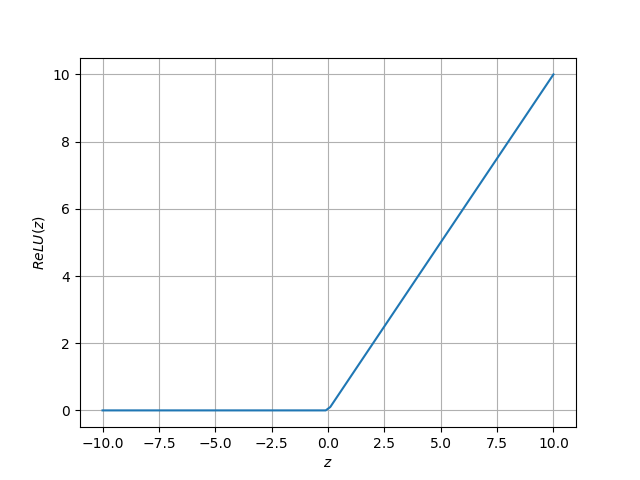
\includegraphics[width=0.5\textwidth]{./figures/ReLU.png}
    \caption{Gràfica de la funció ReLU}
\end{figure}
\begin{comment}
Tot i això, aquesta funció té una desavanantatge; si utilitzen la funció ReLU com a funció d'activació pasarà una cosa, i es que tots els valors negatius són 0, per tant en el procès de retropropagació, explicat a l'apartat \ref{subsec:retropropagació}, no es produeix els valors d'ajust en les neurones negatives. Per solucionar aquest problema s'ha inventat una nova funció que es diu Leaky ReLU. Funciona igual com l funció ReLU, però té un valor determinat per les neurones negatives.

\begin{figure}[h!]
    \centering
    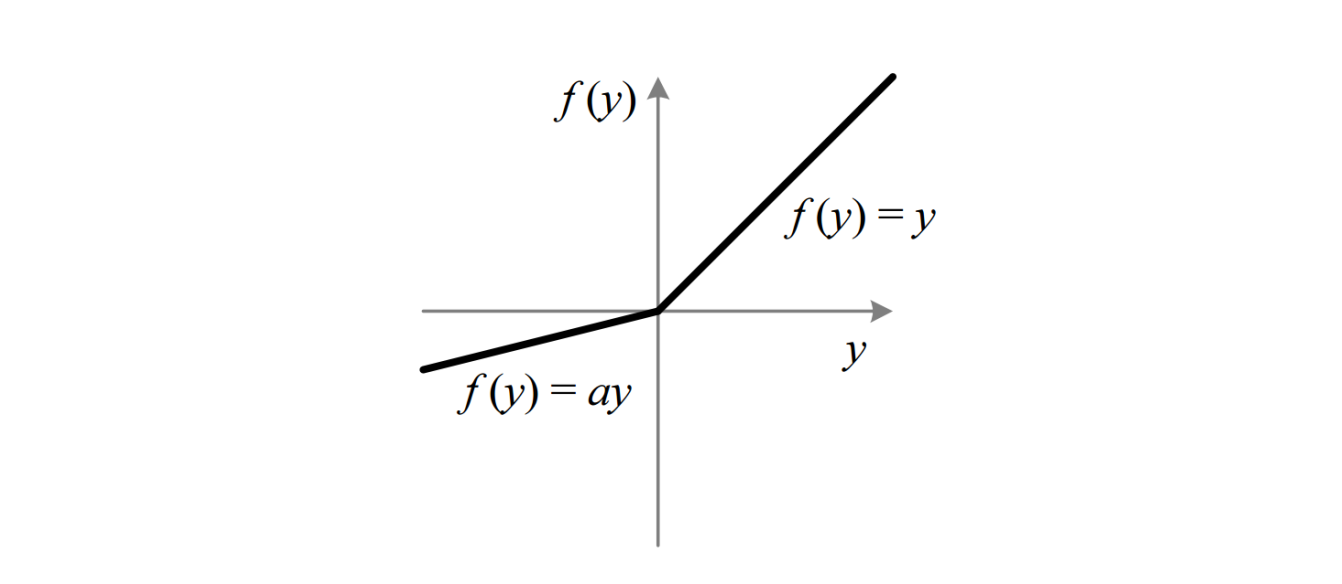
\includegraphics[width=0.5\textwidth]{./figures/leaky_ReLU.png}
    \caption{Gràfica de la funció Leaky ReLU}
\end{figure}
\end{comment}

\item \textbf{Funció Softmax}\\

La funció Softmax és una de les funcions que més s'utilitzen en xarxes neuronals i és especialment útil en el context dels problemes de classificació multiclasse. Aquesta funció opera sobre un vector que representa les previsions de cada classe, calculades per les capes anteriors.

\begin{figure}[h!]
    \centering
    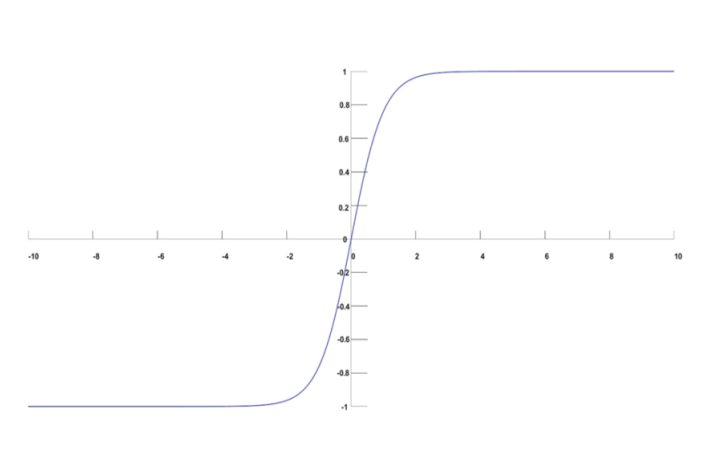
\includegraphics[width=0.5\textwidth]{./figures/Softmax.png}
    \caption{Gràfica de la funció Softmax}
\end{figure}

Per a un vector d'entrada x amb elements x1, x2,..., xC, la funció Softmax es defineix com:
$$[f(x_i) = \frac{e^{x_i}}{\sum_{j=1}^{n} e^{x_j}}]$$

El resultat de la funció Softmax és una distribució de probabilitat de la qual la suma és 1. Cada element del resultat representa la probabilitat que l'entrada pertanyi a una classe determinada. L'ús d'aquesta funció garanteix que tots els valors de la sortida siguin positius. Això és molt important perquè les probabilitats no poden ser negatives.

\begin{figure}[H]
    \centering
    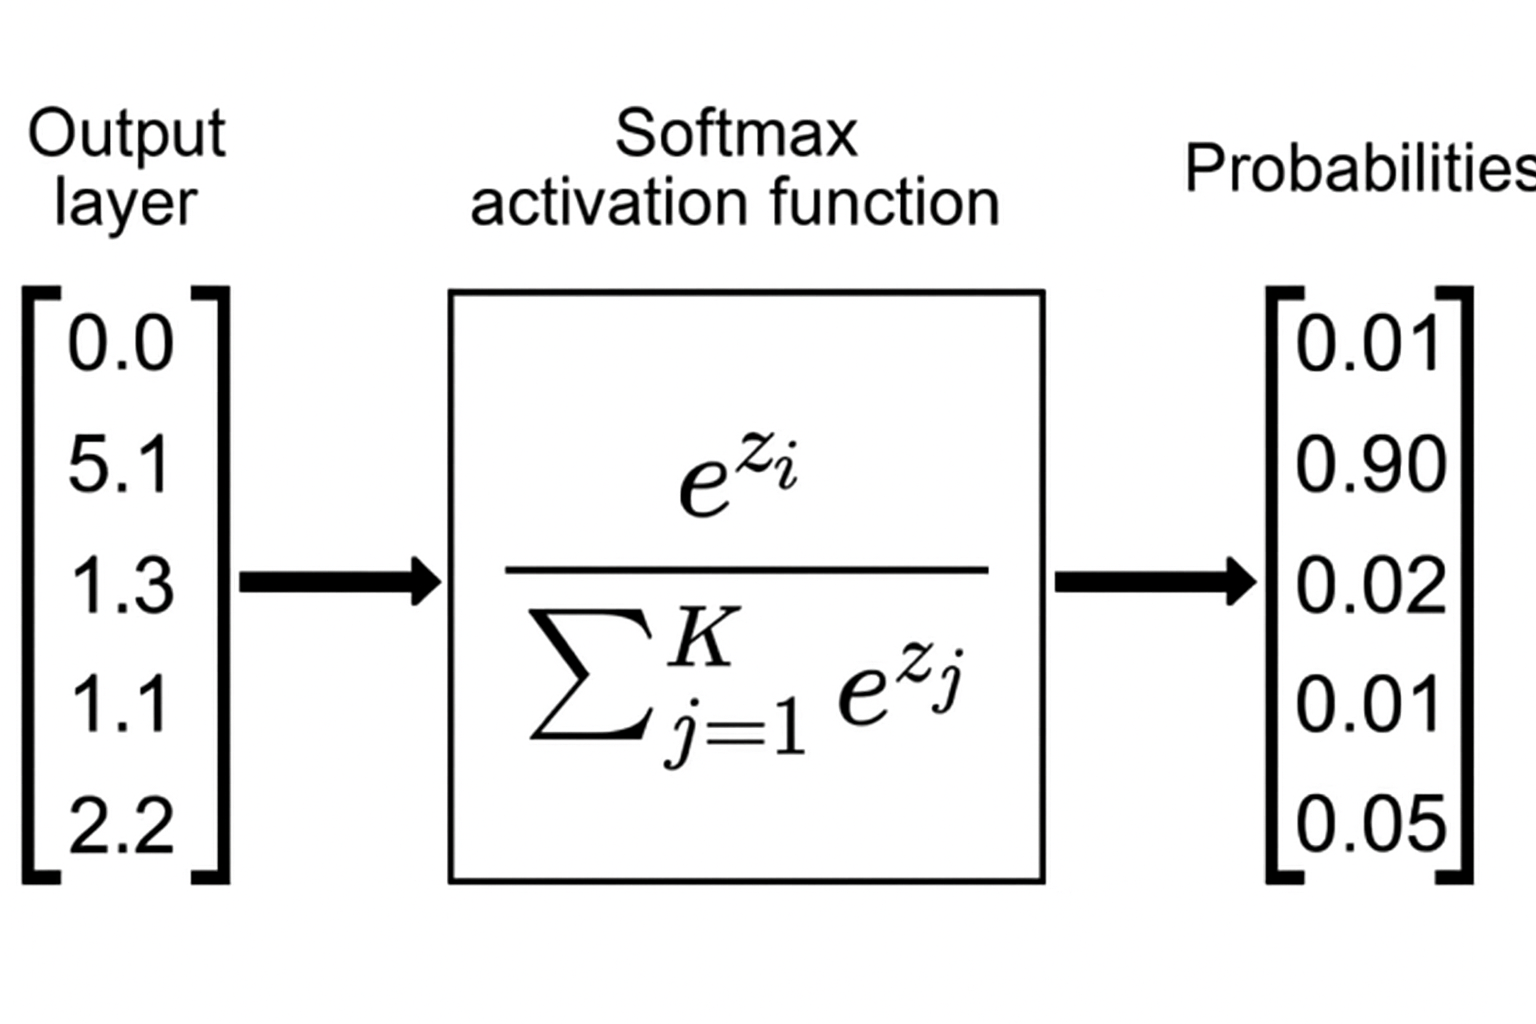
\includegraphics[width=0.5\textwidth]{./figures/representacio_Softmax.png}
    \caption{Representació de la funció Softmax}
\end{figure}

Fonts: ~\cite{Hidden_layer} i~\cite{Jacar}
\end{enumerate}

\section{Com funciona una xarxa neuronal?}\label{sec:3.8}
Ara que sabem quina estructura forma una xarxa neuronal artificial, toca entendre com funciona. Les neurones o nodes són els pilars més importants d'una xarxa neuronal. Cada neurona utilitza l'entrada, la processa fent una suma ponderada entre els pesos i les entrades, després una funció d'activació, i passa la sortida a altres neurones.\\

Les conexions (pesos i biaixos) són la força de connexió entre dues neurones representades per un pes.
\textbf{Els pesos:} Són valors que determinen quanta influència té la producció d'una neurona sobre un altre, marca la importància que té cada neurona.\\

Els biaixos: Són paràmetres addicionals que ajuda a ajustar els valors de les neurones. És un valor capaç d'aprendre com el pes, això vol dir que el model pot utilitzar l'algoritme de retropropagació per a millorar els valors com per exemple els pesos i biaixos.

El umbral: Si la sortida de qualsevol node individual és més gran que el valor del umbral, aquell node s'activarà i envia dades a la següent capa de la xarxa. En cas contrari, no passarà cap dada a la següent capa de la xarxa.\\

Hem de pensar en què cada node individual com el seu propi model de regressió lineal, compost per dades d'entrada, ponderacions, un umbral o un biaix, i una sortida. La fórmula per calcular els valors d'una xarxa neuronal és la següent:

$$[
\sum w_i x_i + \text{biaix} = w_1 x_1 + w_2 x_2 + w_3 x_3 + \text{biaix}
]$$ \\

$w_i$: Pesos\\
$x_i$: Entrades\\

\begin{comment}
Per entendre-ho millor, donarem un exemple: Imagina que vols anar a la platja a fer surf i la teva decisió dependrà d'aquestes 3 preguntes:\\

Hi ha oles?\\
Hi ha poca gent?\\
Hi ha tauros?\\

Analitzarem en detall com funciona un sol node de la xarxa neronal, utilitzant únicament valors binaris (0 y 1) com entrades, 0 voldrà dir ``No'' y 1 ``sí''.
LLavors suposent el següent cas:

$x_1$ = 1, les oles són bones\\
$x_2$ = 0, hi ha molta gent a la platja\\
$x_3$ = 1, Sí que tinc temps\\

Ara, hem d'asignar algunes ponderacions per determinar la importància. Unes ponderacions majors significan que determinades variabbles son més importants per la decisió.

$w_1$ = 5, hi ha d'haveri moltes oles per poder surfejar\\
$w_2$ = 2, no t'importa que hi hagi molta gent\\
$w_3$ = 4, tens pors als taurons \\

Per últim, ambé suposem un valor umbral de 3, ho que es traduiria en un valor de biaix de -3. Amb totes aquestes entrades, ja podem substituir els valors en la nostre fòrmula per obtenir la sortida.
\end{comment}

Fonts: \cite{IMB_Xarxa_neuronal}
%\href{https://aws.amazon.com/es/what-is/neural-network/}{Amazon Web Services} Aquesta pàgina ja no existeix

\subsection{Propagació cap a davant}\label{subsec:propagació}
Durant la propagació cap a davant, les dades ingressen en la xarxa a través de la capa d'entrada i flueixen seqüencialment a través de les capes ocultes fins a la capa de sortida. En cada neurona, els valors d'entrada del model es multipliquen pels seus pesos corresponents i se sumen. Aquesta suma ponderada passarà a través d'una funció d'activació, explicada prèviament a l'apartat \ref{Activació}. Aquest procés continua capa per capa, això acaba conduint cap a la predicció final en la capa de sortida.

Aquest procés és important per les següents raons:
\begin{itemize}
 \item \textbf{Base per l'aprenentatge:} No es pot comprendre com aprenen les xarxes neuronals sense primer entendre com fan prediccions. La programació cap a davant és el requisit previ que s'ha de conèixer per comprendre la \nameref{subsec:retropropagació}, l'algoritme que permet l'aprenentatge.

 \item \textbf{Optimització:} En el cas que una xarxa neuronal no funcioni bé, saber com flueixen les dades per la xarxa t'ajudarà a identificar i solucionar problemes.

 \item \textbf{Disseny del model:} Un disseny eficaç de la xarxa requereix comprendre com es distribueix la informació a través de les configuracions de capes.
\end{itemize}

\section{Retropropagació en les xarxes neuronals}\label{subsec:retropropagació}
Mentre que la programació directa fa prediccions, la retropropagació és la forma en què la xarxa aprèn d'errors. Implica comparar la predicció de la xarxa amb el valor objectiu real i calcular un terme d'error mitjançant una funció d'error.\\
Aquest error es propaga enrere a través de la xarxa, començant des de la capa de sortida. Durant aquest procés, la xarxa ajusta els pesos i els biaixos de cada connexió en funció de la seva contribució a l'error, amb l'objectiu de minimitzar-lo.\\
Aquest procés iteratiu de càlcul d'erros i ajustament de pes permet a la xarxa d'aprenentatge profund millorar gradualment les seves prediccions.\\
El procés de retropropagació es basa en el principi d'optimització del gradient descendent, explicat anteriorment en l'apartat \ref{Algoritme_gradient}, es calculen els gradients d'error respecte als paràmetres de la xarxa en sentit contrari i en cada capa. Per aquesta tasca, s'utilitza l'algoritme de la cadena per propagar l'error cap endarrere des de la sortida fins a l'entrada.

\subsection{Com funcona la retropropagació?}
El funcionament de la retropropagació el podem dividir en 5 fases. Cada una d'aquestes possibilita a la xarxa neuronal aprendre de manera eficient a partir de dades proporcionades. Les fases són les següents:

\begin{itemize}

 \item \textbf{Propagació cap endavant:} Aquesta fase inicial és on s'introdueixen les dades de prova en la xarxa neuronal des de la capa d'entrada fins a la sortida.

 \item \textbf{Càlcul d'error:} Una vegada s'obté la sortida de la xarxa, es compara amb el valor desitjat mitjançant una funció d'error. Aquesta funció quantifica la discrepància que s'ha produït entre la predicció i el valor real.

 \item \textbf{Retropropagació de l'error:} En aquesta fase els gradients de l'error es calculen respecte a cada paràmetre en la xarxa. Com hem dit abans, aquest procés comença de manera inversa a la propagació, des de la sortida fins a l'entrada.

 \item \textbf{Actualització dels paràmetres:} Una vegada que s'ha calculat els gradients de l'error en tots els paràmetres, aquests s'actualitzen. D'aquesta manera, els errors en la predicció es minimitzen de manera gradual en cada iteració de l'entrenament.

 \item \textbf{Configuració de la predicció:} Després de totes les optimitzacions, el mètode de càlcul torna a revisar les entrades de prova. Després de tot això, es busca garantir els resultats esperats.
\end{itemize}
\begin{comment}
\subsection{Avantatges de la retropropagació}
La retropropagació ofereix unes avantatges que l'han convertit en una eina fonamental en l'entrenament de les xarxes neuronals. Les seves avantatges són les seguents:

\begin{itemize}
 \item \textbf{Eficiència en l'optimització de parámetres:} Gracies al càlcul de gradient mitjantçant la regla de la cadena, explicada a l'apartat \ref{subsec:cadena}, la retropropagació facilita l'ajust dels paràmetres d'una xarxa neuronal de manera eficient. Això s'aconsegueix determinant la contribució de cada variable al error total de la xarxa, ho que augmenta notablement a l'hora de fer prediccions precises.
 \item \textbf{Flexibilitat en l'arquitectura:} La retropropagació és compatible en moltes varietats d'arquitectura en les xarxes neuronals, com l'aprenentatge profund amb múltiples capes ocultes. Aquesta característica permet disenys que s'adapten millor a la complexitat de dades i les necesitats de cada tasca.
 \item \textbf{Escalabilitat:} Es posible augmentar la retropropagació perquè traballi amb moltes dades i xarxes neuronas molt grans, ja que hi haurà vegades en que una xarxa pot tindre fins a milions de paràmetres, això exigeix una gestió eficient.
 \item \textbf{Optimització continua:} La retropropagació ofereix la actualització contínua de les variables durant l'entrenament. És un ajust dinàmic important per millorar poc a poc el rendiment de la xarxa amb cada iteració i nous cicles d'aprenentatges.
\end{itemize}
\end{comment}
Fonts: ~\cite{valencia} i~\cite{Retropropagacio}




%
\chapter{Metodologia}
Després d'haver fet la recerca previa, i d'haver decidit fer una xarxa neuronal ``model'' que compleixi tots els requesits que esperavem, ara cal pensar amb quina metodologia podrem aconseguir el nostre objectiu. Per tant vol dir que hem de fer un altre recerca en el que utilizarem les millors eines per fer el Treball de Recerca de manera ràpida i eficient.


Primer ens em fet la pregunta de  sobre quins àmbits hem de recorre, una vegada feta la pregunta ja buscarem les millors eines o mètode que ens ajudarà en cadascún dels àmbits. A continuació farem unes presentacions dels àmbits que vam tractar i les diferents solucions que vam donar i el definitiu.

Per començar tractem  l'apartat \ref{sec:4.1}, que consisteix en com vam estructurar la via de comunicació entre nosaltres i el tutor. A l'apartat \ref{sec:4.2}, tracta de quin editor de text vam escollir, que es un punt crucial per el treball ja que les eines que ens aporta l'editor en si mateix ens pot estalviar molt de temps i convertirlo visualment més accessible. A continuació hi es l'apartat \ref{sec:4.3}, on t'explica la plataforma que hem escollit per l'entorn col·laboratiu. Finalment per poder crear una xarxa neuronal hem d'utilizar un llenguatge de programació i això s'explicarà a l'apartat \ref{sec:4.4}.



\section{Comunicació}\label{sec:4.1}
Com que som dos persones fent el treball amb un tutor, ens és fonamental tenir una bona via comunicativa. Per tant, hem acollit diferents maneres de comunicació. Ara bé no em pogut registrar tots els registres que hem tingut però la gran majoria s'ha pogut conservar.\\
D'aquí cap avall explicarem les diferents maneres de comunicació utilizades en l'elaboracio d'aquest treball:\\
\subsection{Full de Calculs}
Hem realitzat diverses reunions amb el tutor, i la via que vam utilitzar per configurar l'horari de les quedades és a travès d'un full de càlcul. En aquestes quedades ens em organitzat el treball i ens em quedat amb els diferents mètodes que utilizariem per el trebal, el tutor ens arregla qualsevol tipus de problema, i la instalació dels programes necessaris.
\subsection{Correu Electrònic}
L'eina que vam utilizar a distància és el servei de correu electrònic Gmail. Vam fer ús d'aquest aparell per el fet de que és simple i eficient, i té una gran memòria d'emmagatzament per conservar tots els correus que ens hem fet.
Les converses fetes per el correu electrònic ha sigut la principal via de comunicació que em establert, per la facilitat i l'eficiència que ens aporta. Per tant, el tema ensenyament i dubtes simples o feiem tot per gmail.

\subsection{Git}
També amb l'ajuda del Git, un software que ens va ajudar a guardar tots els canvis que hem anat fent durant el treball de recerca. Vam  establir una comunicació diària amb el progrés del treball, deixant comentaris dels canvis i adaptacions que vam anar fet.


\section{Editor de text i processador de text}\label{sec:4.2}
Per aconseguir una bona presentació de TR, haviem d'escollir o un editor de text o un processador. Tant l'editor com el processador són per crear documents, pero cadascún te les seves funcions.\\
L'editor de text, és tal com el seu nom, serveix per editar els documents. És molt simple i això genera inconvenients, com per exemple no poder utilizar formats avançat o una personificació. Però, les avantatge d'aquest és que pots tenir la capacitat de navegar rapidament de fitxer en fitxer, facilita la codificació i té compabilitat amb tots els tipus de llenguatge. És l'ideal per programadors.\\
Un processador de text són tipus de programes més elaborats i més complexos. Com que són programes amb tanta complexibilitat, et dona accès a formats avançat, utilitzat per a documents professionals com currículums, llibres i d'altres més, també et donen tot tipus d'opcions col·laboratives com disseny de pàgina, correció gràfica i molt més.\\
Per a la part teòrica del nostre projecte sobre la Intel·ligència Artificial, vam seleccionar el format PDF degut a:
\begin{enumerate}
 \item Connexió segura i estable: Permet l'accés sense la dependència d'una connexió a Internet constant.
 \item Baixos requisits de recursos: Pot obrir-se en gairebé qualsevol dispositiu sense necessitat de programes específiques.
 \item Portabilitat: Manté el format independentment del sistema operatiu utilitzat.
 \item Multifuncionalitat: Admet text, fórmules matemàtiques, imatges i codi de programació integrat.
\end{enumerate}
L'estalvi de temps va ser un factor decisiu, ja que evita problemes de compatibilitat entre fórmules matemàtiques, imatges i el format del document.
En la nostra recerca d'eines que satisfacin tots els requisits, vam identificar dos tipus principals de processadors: Una que es deia WYSIWYG (What You See Is What You Get) i l'altre el WYSIWYM (What You See Is What You Mean). Ara donarem una explicació de les advantatges i desavantatges que tenen:
\subsection{What You See Is What You Get(WYSIWYG)}
WYSIWYG, es refereix a un tipus de processador que permet als usuaris veure en temps real el resultat final del document o disseny mentre editen, sense la necessitat de coneixer el codi o llenguatges de marcatges. Aquests tipus d'editors poden ser tant com el microsoft word o Google drive.

\textbf{Característiques}:
\begin{itemize}
 \item \textbf{Interfície visual:} Els canvis de format (negretes, taules, imatges) es fan mitjançant eines gràfiques, no mitjançant codi.
 \item \textbf{Generació automàtica de codi:} El programa crea el codi subjacent (HTML, CSS, etc.) sense que l'usuari hi intervingui directament.
 \item \textbf{Ús generalitzat:} S'utilitza en àmbits com l'edició web, el disseny gràfic i la publicació digital.
\end{itemize}
Avantatges:
\begin{itemize}
\item \textbf{Edició visual intuïtiva:} Permet ajustar el format directament (arrossegar imatges, canviar fonts amb clics).
 \item Ideal per a usuaris sense coneixements tècnics.
\item \textbf{Resultat immediat:} No cal compilar, els canvis es veuen al moment.
\item \textbf{Eines integrades:} Funcions com correcció ortogràfica, taules gràfiques, o opcions de disseny accessibles des del menú
\item \textbf{Millor per a maquetació complexa:} Documents amb molts elements gràfics (pòsters, fulls informatius)
\end{itemize}
Desavantatges:
\begin{itemize}
 \item \textbf{Poca precisió en contingut tècnic:} Fórmules matemàtiques o codis es poden deformar-se a l'hora de canviar el format.
 \item \textbf{Errors en documents llargs:} El format manual pot provocar errors (salt de pàgina, numeració desorganitzada).
 \item \textbf{Dependència del programa:} Si s'obre en un altre software, el disseny pot variar.
 \item \textbf{Control de versions complicat:} Difícil treballar en equip sense conflictes de format.
\end{itemize}

\subsection{What You See Is What You Mean(WYSIWYM)}\label{subsec:4.2.2}
WSYSIWYM, es refereix a un tipus de processador que es centra en l'estructura del contigut, no en la seva aparença visual immediata, l'usuari marca el text segons la seva funció (títol, secció, cita i d'altres més) i el format final s'aplica mitjançant un full d'estil com css o Latex.
Avantatges:
\begin{itemize}
\item \textbf{Precisió en elements tècnics:} Fórmules matemàtiques, codi o referències es gestionen amb sintaxi clara.
\item \textbf{Consistència automàtica:} L'estil s'aplica globalment.
\item \textbf{Lleuger i portable:} Els fitxers són de text pla.
 \item \textbf{Ideal per a treball en entorns col·laboratius:} Es pot actualizar amb git i fusionar sense haver de canviar el format.
\end{itemize}
Desavantatges:
\begin{itemize}
\item \textbf{Corba d'aprenentatge:} Cal aprendre una sintaxi específica.
 \item \textbf{Previsualització no immediata:} En LaTeX, cal compilar; en Markdown, cal un renderitzador.
 \item \textbf{Limitacions en disseny gràfic:} Personalització avançada (ex: posicionament exacte d'imatges) requereix codi addicional.
\end{itemize}

\begin{table}[h!]
\begin{tabular}{|l|l|l|}
\hline
\textbf{Aspecte} & \textbf{WYSIWYG} & \textbf{WYSIWYM} \\ \hline
\textbf{Enfocament} & Aparença visual immediata & Estructura semàntica del contingut \\ \hline
\textbf{Exemples} & Microsoft Word, WordPress & LaTeX, LyX \\ \hline
\textbf{Usuaris} & No tècnics, dissenyadors &  Acadèmics, desenvolupadors tècnics \\ \hline
\textbf{Control} &  Limitada (codi generat automàtic) & Alt (definició manual de l'estructura) \\ \hline
\end{tabular}
\caption{Comparativa entre WYSIWYG i WYSIWYM}
\end{table}



font(WYSIWYG): (\href{https://es.wikipedia.org/wiki/WYSIWYG}{Wikipedia} \href{https://es.wikipedia.org/wiki/WYSIWYG}{Arimetrics} \href{https://www.wix.com/encyclopedia/definition/wysiwyg}{Wix}).
font(WYSIWYM): (\href{https://en.wikipedia.org/wiki/WYSIWYM}{Wikipedia} \href{https://en.ryte.com/wiki/WYSIWYG/}{Ryte WIKI}).



\subsection{\LaTeX}
\begin{comment}
% l'entorn figure et numera la figura i et permet posar una nota al peu de la figura, però costa controlar la posició
\begin{figure}[h!]
    \centering
    
\includegraphics[width=0.5\textwidth]{./figures/latex.png}
    \caption{Logo del Latex}
\end{figure}%

% si ho fas d'aqesta manera
\begin{center}
    
\includegraphics[width=0.75\textwidth]{./figures/latex.pdf}
\end{center}
\end{comment}

\LaTeX, és un tipus de WYSIWYG, on s'enfoca en l'estructura lògica, no la visual, tal com vam mencionar en l'apartat \ref{subsec:4.2.2}. LaTeX és un sistema de composició tipogràfica d'alta qualitat, especialment dissenyat per a la creació de documents acadèmics, tècnics i científics. A diferència dels processadors de text tradicionals com Microsoft Word, LaTeX es basa en codi per estructurar el document, separant el contingut de la seva presentació visual. Va ser desenvolupat per Leslie Lamport en 1984 com un conjunt de macros per al sistema TeX de Donald Knuth. La raó principal de la seva creació va ser la impotència dels processadors de text de l'època per compilar fórmules matemàtiques avançades i gestionar documents complexos amb precisió tipogràfica. És per aquesta raó la qual el vam escollir com a processador per satisfer els requeriments que demanem. Per més informació o dubte podeu consultar el manual de latex:  \href{https://manualdelatex.com/}{Manual de LaTeX}
\subsection{Kile}
Kile es un editor especific del \LaTeX que funciona en els sistemes operatius tant Linux, Windows com Apple Macintosh. L'editor va ser desenvolupat per la comunitat  \nameref{subsec:KDE} en que ofereix diverses eines avannçades per a l'edicio de LaTeX. No és l'únic editor que existeix, però és el que més ens convé per el fet de que sigui creat per documents acadèmics i científics.\\

Avantatges:
\begin{itemize}
\item \textbf{Entorn integrat complet:} Kile ofereix tot ho necessari per treballar amb LaTeX en una sola interfície, incloent editor, compilador, visualitzador i gestor de referències
\item \textbf{Altament configurable: } Permet afegir botons a la barra d'eines per executar scripts personalitzats i automatitzar tasques complexes.
\item \textbf{Feedback WYSWYG:} Et dona una sensació quasi WYSWYG, gracies als visualitzadors que els té integrades en que pots veure els canvis en temps reals.
\item \textbf{Eines avançades d'edició:} Té autocompletador de comandes, accés ràpid a símbols matemàtics, navegacions ràpides per seccions.
\end{itemize}
Desavantatges:
\begin{itemize}
\item \textbf{Nivell d'apranentatge:} Costa molt d'aprendre l'interfície si no estas familialitzat amb KDE.
\item \textbf{Configuració inicial:} Requereix molts tipus de configuracions externs per tal d'arrenca.
\end{itemize}

Ara mostrarem una taula de comparació respecte els altres editors:
LyX és més adequat per a principiants gràcies a la seva interfície WYSIWYG. No obstant, Kile es més flexible per als usuaris avançats i te més control en els codis i funcions. \\
%Taula 1
\begin{table}[h!]
 \begin{tabular}{|l|l|l|}
\hline
 \LaTeX & \textbf{Kile} & \textbf{LyX} \\ \hline
 \textbf{Facilitat d'ús} &  & X \\ \hline
 \textbf{Control i Flexibilitat} & X & \\ \hline
 \textbf{Visualització en temps real} & & X \\ \hline
\end{tabular}
\end{table}

TeXmaker i TeXstudio comparteixen moltes similituds amb Kile en termes de funcionalitat i d'interfície. \\

%Taula 2
\begin{table}[h!]
 \begin{tabular}{|l|l|l|}
\hline
 \LaTeX & \textbf{Kile} & \textbf{TeXmaker i TeXstudio} \\ \hline
 \textbf{similitud de funcionalitat} & - & - \\ \hline
 \textbf{Integració KDE} & X & \\ \hline
 \textbf{Disponibilitat dels sistemes operatius} & X &  \\ \hline
 \end{tabular}
\end{table}

Gummi és un editor molt més simple que Kile, amb previsualització en temps real però amb moltes menys funcionalitats. És bo per a documents simples però per a projectes complexos no. \\
%Taula 3
\begin{table}[h!]
 \begin{tabular}{|l|l|l|}
\hline
 \LaTeX & \textbf{Kile} & \textbf{Gummi} \\ \hline
 \textbf{complexibilitat:}  & X &  \\ \hline
 \textbf{Previsualització} &  & X \\ \hline
 \textbf{funcionalitat} & X &  \\ \hline
 \end{tabular}
\end{table}

Per més informació en qüestió de comparació podeu fer una consulta a les següents pagines: \href{https://osluca.uca.es/noticia/cinco-editores-de-latex-libres/}{5 editors de LaTeX} \href{https://latex.org/forum/viewtopic.php?t=208}{Analisí detallada de Kile i d'altres editors}
Fonts: \href{https://iloo.wordpress.com/2010/10/20/kile-otro-editor-latex/}{Experiencia Personal de l'us Kile} \href{https://www.kdeblog.com/editor-de-latex-para-kde-kile.html}{Descripcio de Característiques Kile}

\subsection{KDE}\label{subsec:KDE}
El nom "KDE" originalment sí que era un acrònim de "K Desktop Environment" (des de la seva creació el 1996), però a partir del 2009, la comunitat va decidir deixar de considerar-lo un acrònim i utilitzar-lo simplement com un nom propi per representar:
\begin{itemize}
 \item L'entorn d'escriptori.
 \item La comunitat global que desenvolupa programari lliure.
 \item Tots els projectes relacionats.
\end{itemize}
Font:\href{https://ca.wikipedia.org/wiki/KDE}{Wikipedia}

\subsubsection{Programari lliure}

El programari (o software en anglès) és el conjunt de programes informàtics, procediments i documentació que permeten a un ordinador realitzar tasques específiques. És la part interna d'una computadora ,a difèrencia del hardware que és l'extern, el software és part física.

Un programari es considera Free software quan respecta les quatres llibertats fonamentals definides per la Free Software Foundation (FSF):
\begin{enumerate}
 \item  \textbf{Llibertat 0:} Executar el programa amb qualsevol propòsit.
 \item  \textbf{Llibertat 1:} Estudiar i modificar el codi font (requereix accés al codi)
 \item  \textbf{Llibertat 2:} Redistribuir còpies per ajudar altres usuaris.
 \item  \textbf{Llibertat 3:} Millorar el programa i compartir les modificacions.
\end{enumerate}

Mapa conceptual del Free software:
\begin{center}
\hspace{-27mm}
 \includegraphics[scale=0.1]{./figures/mapa.png}
\end{center}

Font:\href{https://www.fsf.org/}{Free Software Foundation}

\subsubsection{L'entorn d'escriptori}
Un entorn d'escriptori en sistemes operatius és la interfície gràfica que permet als usuaris interactuar amb l'ordinador. Inclou elements com finestres, icones, panells, fons de pantalla i eines de gestió d'arxius.A continuació, mostrarem els principals entorns que n'hi ha:
\begin{enumerate}
 \item KDE Plasma
 \begin{itemize}
  \item \textbf{Característiques: } Altament personalitzable, amb temes globals, widgets i configuració avançada.
  \item \textbf{Recomanat per:} Usuaris que volen control total sobre l'aparença i el flux de treball.
 \end{itemize}

 \item GNOME
 \begin{itemize}
  \item \textbf{Característiques:} Disseny minimalista i enfocat en la productivitat. Compatible amb extensions per ampliar funcionalitats.
  \item \textbf{Recomanat per: }  Usuaris que prefereixen una experiència neta i senzilla.
 \end{itemize}


 \item XFCE
\begin{itemize}
  \item \textbf{Característiques:} Lleuger i ràpid, ideal per a maquinari antic o limitat.
  \item \textbf{Recomanat per: } Usuaris que busquen eficiència sense sacrificar funcionalitats bàsiques .
 \end{itemize}

 \item Cinnamon
\begin{itemize}
  \item \textbf{Característiques:} Interfície tradicional similar a Windows, amb personalització mitjana.
  \item \textbf{Recomanat per: } Usuaris que provenen de Windows i busquen una transició suau.
 \end{itemize}

\end{enumerate}


Fonts:\href{https://dev.to/xploitcore/kde-vs-gnome-vs-others-choosing-the-best-linux-desktop-environment-in-2025-ab5}{Dev} \href{https://planet.communia.org/index.php/en/node/77}{Planet}



\section{Entorn col·laboratiu}\label{sec:4.3}
A l'hora de crear un projecte en equip, pot arribar a ser complicat treballar amb 2 o més membres del grup a la vegada en els seus respectius dispositius si no s'escull una eina col·laborativa adequada, sobretot si s'està treballant amb molts fitxers. Pot haver problemes alhora de intercanviar o que sol pugui estar un membre traballant en un fitxer fa que sigui un absolutament caos.
\subsection{Google Drive}
Google Drive és una plataforma de Google que ofereix eines gratuïtes com un processador de text (Docs) i un entorn col·laboratiu. Tot i ser senzill i eficient, té algunes limitacions importants que hem de considerar:
\begin{itemize}
 \item \textbf{Poc control en el procés col·laboratiu:} És difícil gestionar canvis simultanis o conflicts entre versions.
 \item \textbf{Limitacions en el control de versions:} No permet controlar detalladament els canvis que es fan i registrar.
 \item \textbf{Falta de privadesa:} Google té accés als teus arxius, cosa que pot ser un problema per a dades sensibles.
\end{itemize}
Aquestes limitacions fan que Google Drive no sigui l'opció ideal per el nostre TR la qual cosa ens fara escollir l'altre alternativa que teniem, el \nameref{subsec:Git+GitHub+Vim}.
\subsection{Git+GitHub+Vim}\label{subsec:Git+GitHub+Vim}
Git és un sistema de control de versions que ofereix:
\begin{itemize}
 \item Historial dels canvis.
 \item Branques per desenvolupar diferents funcionalitat sense afectar la versió principal.
 \item Control total dels canvis
 \item Control i revisió de codi
\end{itemize}
El principal desavantatge que té el Git és que, per si sol, no està optimitzat per a la col·laboració en equips grans. Pero aquí entra en acció el GitHub, que complementa Git amb:
\begin{itemize}
\item \textbf{Repositoris}
 \item \textbf{Git pull,commit,push:} Dona la possibilitat de poder discutir les versions abans de pujarlo a la original.
 \item Solucions als conflictes de versions amb l'ajuda del \nameref{subsubsec:Vim}.
 \end{itemize}

\textbf{Avantatges:}

\begin{itemize}
 \item \textbf{Copia de seguretat:} Cada usuari té una copia de seguretat del servidor principal, en el cas d'errors o corrupció, sempre el pots reemplaçar-lo per el servidor principal.
 \item \textbf{Garantia de dades:} El model de dades que utilitza Git garantitza la integritat ciptográfica de cada bit del teu projecte. Cada arxiu es recupera mitjançant la seva suma de comprobació quan es torna a desgarregar-se. Es imposible obtenir res de Git que no sigui els bits exactes que s'ha integrat.
 \item \textbf{Àrea de preparació:} Una cosa que diferència a Git d'altres eines es que es posible preparar alguns dels teus arxius i confirmar-los sense confirmar tots els altres canvis que s'han fet en els altres arxius, això et permet preparar nomès algunes parts d'un arxiu modificat i es realitza amb el commandament git commit ``nom de l'arxiu''. Git també et dona la opció d'ignorar aquesta característica i confirmar tots els canvis que s'han fet, afegint un ``-a'' al final del commandament.
 \item \textbf{Eficiència de Git:} Git no depèn d'internet per la majoria de les operacions, totes les accions principals (veure l'historial, fer commits) es fan en localment. Git està programat en llenguatge C, això permet a Git realitzar les tasques amb molta rapidesa encara que es treballi amb molts fichers.
\end{itemize}
Més informació en: \href{https://git-scm.com/about/branching-and-merging}{Pagina oficial del Git}

\textbf{Desavantatges:}
\begin{itemize}



\item \textbf{Corba d'aprenentatge pronunciada}: Git té un model conceptual complex (working directory, staging area, repositori local/remot) que requereix temps per assimilar. Operacions bàsiques com merge/resolucions de conflictes poden resultar difícils per a principiants.

      \begin{enumerate}
        \item \textbf{Working directory:}
         \begin{itemize}
            \item La carpeta local del projecte on treballes i fas canvis als fitxers.
            \item Modifiques, elimines o crees nous arxius
            \item Git analiza aquest aquest directori per fer la comparació dels canvis respecte l'ultima versió
          \end{itemize}

        \item \textbf{Staging Area:}
         \begin{itemize}
            \item És el cache del Git
            \item Una zona intermedia on inclous els canvis propers que vols fer
          \end{itemize}

        \item \textbf{Repositori Local:}
        \begin{itemize}
            \item És la base de dades completa de Git que es troba a la teva màquina (dins de la carpeta .git)
            \item Conté tot l'historial de commits, branques, tags del Git
            \item Els canvis del Staging Area, es guarden permanent aqui
          \end{itemize}
        \item \textbf{Repositori Remot:}
        \begin{itemize}
            \item És una copia del repositori en un servidor (GitHub, GitLab, Bitbucket)
            \item Serveix per compartir codis i funciona com a entorn col·laboratiu
            \item És utilizen comandes git push(Pujar canvis) i git pull(Baixar canvis)
          \end{itemize}
       \end{enumerate}


\item \textbf{Problemes amb fitxers molt grans}: Git no està optimitzat per a fitxers binaries de gran mida (vídeos, imatges, bases de dades). El rendiment es degrada significativament i el repositori pot inflar-se massa.

\item \textbf{Gestió complicada de credencials}: Git no gestiona de forma òptima les credencials.

\item \textbf{Problemes de rendiment en repositoris molt grans}: En repositoris amb milers de commits o arxius, certes operacions (com git status o git checkout) poden tornar-se lentes.

\item \textbf{Comandes}: Els comandes reben nom contraintuïtiu io la sintaxi varia segons l'operació.
\end{itemize}
Fonts:\href{https://ieeexplore.ieee.org/document/8259410}{Comparacions entre control de versions} \href{https://stevebennett.me/2012/02/24/10-things-i-hate-about-git/}{bloc de critica d'un desenvolupador}
\subsubsection{Vim}\label{subsubsec:Vim}
Vim (Vi IMproved) és un editor de text avançat, lliure i de codi obert, basat en l'editor clàssic vi. És conegut per ser multiplataforma i també la seva eficiència, personalització i ús sense ratoli, sent popular entre programadors i usuaris tècnics. Aquest editor de text consta de 4 modes amb diferents funcionalitats:
\begin{itemize}
 \item \textbf{Mode Estandard:} Per navegar i executar ordres
 \item \textbf{Mode Insert:} Per escriure text
 \item \textbf{Mode Visual:} Per seleccionar bloc de text
 \item \textbf{Mode Command} Per executar comandes complexes
\end{itemize}
Fonts:\href{https://www.vim.org/}{Pagina oficial del Vim} \href{https://vimhelp.org/}{Documentacio del Vim}
\section{Llenguatge de programació}\label{sec:4.4}

El llenguatge de programació que vam decidir per fer la part pràctia del treball va ser Python. Python és un llenguatge de programació que va ser creat en 1989 per Guido van Rossum , un informàtic neerlandès. Aquest llenguatge és conegut per la seva simple sintaxi, comparada amb altres llenguatges com JavaScript o C++ que són més complicats, python facilita l'aprenentatge pels usuaris que començen a apendre a programar desde 0.

\subsection{Python}
La raó principal per la que vam escollir aquest llenguatgera per les avantatges seguents:

\textbf{Avantatges}
\begin{itemize}
 \item \textbf{No cal compilar:} No és necesari compilar en Python, un cop que tens el codi, s'executa directament.
 \item \textbf{Llibreries} Python té una gran quantitat de llibreries molt útils com ``TensorFlow'' o numpy, aquestes llibreries estalvien moltes línies de codi a l'hora de programar una xarxa neuronal.
 \item \textbf{Identificació d'errors} Encara que altres llenguatges també poden identificar-te els erros, Python t'ho explica de manera més clara i precisa, estalviant-te el temps d'anar línea per línea buscant l'error.
 \item \textbf{Sintaxi:}La seva sintaxi clara i llegible que està explicada a l'apartat \ref{4.4.2} és ho que fa que aquest llenguatge sigui fàcil d'apendre quan un comença a programar desde 0.
\end{itemize}

Malgrat totes aquestes avantatges, Python tambè té unes porques desaventatges que hem de tenir present.

\textbf{Desavantatges:}
\begin{itemize}
 \item \textbf{Limitacions de rendiment:} La naturalesa interpretada de Python significa que és més lent que altres llenguatges. La causa d'això és que Python es tradueix a codi màquina línea per línea durant l'execució del codi, cosa que afegeix un temps de processament.
 \item \textbf{Consum de memoria:} Gràcies a la bona fexibilitat d'aquest llenguate fa que l'ordinador requereixi un major consum de memòria, un consum excesiu de la memoria pot causar relentizació en el programa i bloquejar-lo. Per tant es recomendable tenir un ordinador o portatil decent que pugui executar correctament Python.
\end{itemize}

\subsection{Sintaxi}
Acabem d'explicar que la sintaxi de Python és simple, però què diferencia aquesta sintaxi d'altres llenguatges? La principal raó és que el seu format de codi és visualment ordenat i utilitza paraules clau de l'anglès. A diferència d'altres llenguatges, no utilitza claudàtors per determinar blocs, com per exemple les sentències ``if, else'':


\begin{table}[h!]
\centering
\begin{tabular}{|p{7cm}|p{7cm}|}
\hline
\textbf{Condicions en C} & \textbf{Condicions en Python} \\ \hline

\begin{minipage}[t]{\linewidth}
\begin{lstlisting}[language=C]
#include <stdio.h>

int main() {
    int numero = 5;

    if (numero > 0) {
        printf("És >0.\n");
    } else {
        printf("\`És <0.\n");
    }
    return 0;
}
\end{lstlisting}
\end{minipage}
&
\begin{minipage}[t]{\linewidth}
\begin{lstlisting}[language=Python]
numero = 5

if numero > 0:
    print("És positiu.")
else:
    print("És negatiu.")
\end{lstlisting}
\end{minipage}
\\ \hline
\end{tabular}
\caption{Comparació de condicions en C i Python}
\end{table}

En aquesta taula podem veurem la diferència de sintaxi que té cada llenguatge, en aquest cas podem apreciar que C és mès llarg que python i que requereis més commandaments i línies de codi. A continuació mostrarem una taula resumida d'aquestes diferències.

\textbf{Resum de diferències:}
\begin{table}[h!]
\centering
\begin{tabular}{|l|l|l|}
\hline
\textbf{Concepte} & \textbf{C} & \textbf{Python} \\
\hline
Terminador de línia & \verb|;| obligatori & No és obligatori \verb|;| \\
\hline
Agrupació de blocs & \{ \} & Espai en blanc \\
\hline
Condició & \verb|if (condició)| & \verb|if condició:| \\
\hline
Estructura & Requereix el script \verb|main()| & Script directe \\
\hline
Librerías & \verb|#include <stdio.h>| & No requereix per \verb|print()| \\
\hline
\end{tabular}
\caption{Resum de les diferències}
\end{table}













%
\chapter{Xarxa Neuronal}
\section{Introducció}\label{sec:intr}
En iniciar la part pràctica del treball vam decidir crear tres tipus de xarxes neuronals: una \nameref{sec:10}, una altra \nameref{sec:11} i, finalment, una \nameref{sec:12}.

En aquest capítol explicarem com vam elaborar cadascuna d’aquestes xarxes neuronals i, a més, compararem les dues formes de desenvolupament en una \nameref{sec:op}.

Per facilitar l’organització del treball, ens hem repartit les tasques: un membre de l’equip s’ha encarregat de la xarxa neuronal implementada amb llenguatge de programació Python, mentre que l’altre ha treballat una xarxa neuronal feta amb fulls de càlcul. Finalment, hem elaborat conjuntament la taula de comparació, intercanviant perspectives, i també hem treballat plegats la xarxa neuronal del cas real.

Les nostres pràctiques consisteixen en recopilar una sèrie de dades d'alumnes mitjançant una enquesta feta per nosaltres amb la finalitat de crear una Xarxa neuronal que pugues predir la nota final de cada alumne. Les preguntes fetes en el formulari són sobre la matèria de matemàtiques i són les següents:
\begin{itemize}
 \item Realització de deures
 \item Hores d'estudis (semanal)
 \item Hores de section
 \item Interès en la matèria
 \item Nota del segon trimestre
 \item Nota del tercer trimestre
 \item Nota final
\end{itemize}
Com es pot veure, les preguntes d'aquest formulari estan relacionades amb el rendiment d'estudis dels alumnes, i s'envia als estudiants que tingues l'assignatura matematiques.


Després de les prediccions, compararem la xarxa neuronal feta amb python y la del full de càlcul i veurem quina de les dos té més precisió.

\section{Xarxa neuronal de regressió}\label{sec:op}
Una intel·ligència artificial és un camp molt extens i, dins d’aquest, les xarxes neuronals també representen una branca àmplia i complexa.
En el nostre context utilitzarem un tipus concret de xarxa neuronal per a la pràctica: les \textbf{xarxes neuronals de regressió}.

Una xarxa neuronal de regressió, a diferència d’una de classificació, té una sortida de tipus lineal que permet predir un valor numèric continu. Aquest tipus de xarxes requereixen un conjunt de dades prou extens i ben estructurat per poder aprendre les relacions entre les variables d’entrada i generar una estimació fiable.

A continuació es mostra un esquema representatiu d’una xarxa neuronal de regressió:

\begin{figure}[h!]
\centering
\begin{tikzpicture}[scale=1, transform shape]

% Input layer
\node[circle, draw, minimum size=1cm] (I1) at (0,2) {$x_1$};
\node[circle, draw, minimum size=1cm] (I2) at (0,0) {$x_2$};
\node[circle, draw, minimum size=1cm] (I3) at (0,-2) {$x_3$};

% Hidden layer
\node[circle, draw, fill=gray!10, minimum size=1cm] (H1) at (3,2) {};
\node[circle, draw, fill=gray!10, minimum size=1cm] (H2) at (3,0) {};
\node[circle, draw, fill=gray!10, minimum size=1cm] (H3) at (3,-2) {};

% Output layer
\node[circle, draw, fill=blue!10, minimum size=1cm] (O1) at (6,0) {$\hat{y}$};

% Connections input -> hidden
\foreach \i in {1,2,3}
  \foreach \h in {1,2,3}
    \draw[->] (I\i) -- (H\h);

% Connections hidden -> output
\foreach \h in {1,2,3}
  \draw[->] (H\h) -- (O1);

% Labels
\node at (0,3) {Entrades};
\node at (3,3) {Capa oculta};
\node at (6,1) {Sortida (regressió)};

\end{tikzpicture}
\caption{Esquema d’una xarxa neuronal de regressió}
\end{figure}

\section{Xarxa Neuronal amb llenguatge de programació}\label{sec:10}
En aquest apartat explicarem pas a pas de com vaig crear el nostre xarxa neuronal de regressió amb un llenguatge de programació.

\subsection{De celcius a fahrenheit}

Abans de començar a treballar amb la xarxa neuronal definitiu, vaig voler fer una de més simple per tal de coneixer amb més profunditat de com funciona una xarxa neuronal de regressió; en aquest cas he escollit un transformador d'unitats de temperatura, de celcius (\textbf{Unitat de temperatura basada en el punt de fusió de l'aigua}) a fahrenheit (\textbf{Sistema d'unitat basada en el punt d'ebullició i solidificació de l'aigua}). Per crear aquesta xarxa vaig escollir el Python com a llenguatge de programació, i el motiu esta explicat en l'apartat \ref{sec:4.4}.\\


Per començar, importo el framework i la biblioteca de Python que són les bases de dades necessàries per a la creació de la xarxa neuronal: \texttt{TensorFlow} (\textbf{framework}) i \texttt{{numpy}} (\textbf{biblioteca}). Com podeu veure, he creat uns \textit{abrevacions} per a poder-los cridar més fàcilment quan els necessiti.

\begin{itemize}
 \item \textbf{TensorFlow: } TensorFlow és un tipus de framework en que ofereix eines per crear i entrenar models de Ml (Machine learning) i Dl (Deep learning), biblioteques per programar xarxes neuronals i altres algoritmes, Compatibilitat amb GPU i TPU per accelerar càlculs, TensorBoard per visualitzar i monitorar entrenaments, Models preentrenats i repositoris, APIs (Application Programming Interface) en diversos llenguatges.
 \item \textbf{numpy: } numpy és una biblioteca científica per treballar amb vectors i matrius.
\end{itemize}
\begin{figure}[H]
    \centering
    
\includegraphics[width=0.5\textwidth]{./figures/1.png}
    \caption{Framework i biblioteca del Python}
\end{figure}


Agafo les paraules \textbf{celsius} i \textbf{fahrenheit} i les defineixo com a variables amb un signe \texttt{=}. Després poso \texttt{np} per indicar la biblioteca, seguit de \texttt{.array()} per especificar que és una llista. Dins dels parèntesis hi poso \texttt{[ ]} i a dins, els diferents valors de temperatura. Finalment, afegeixo el paràmetre \texttt{dtype=float} per indicar que es tracta de dades numèriques decimals.

Repeteixo el mateix procés amb \textbf{fahrenheit}, però en aquest cas les dades no poden ser arbitràries, sinó que han de ser les temperatures corresponents a les de \textbf{celsius} convertides a Fahrenheit. D’aquesta manera, la xarxa neuronal pot entendre la relació entre les dues sèries de dades.


\begin{figure}[H]
    \centering
    
\includegraphics[width=0.5\textwidth]{./figures/2.png}
    \caption{Agrupació de dades amb numpy}
\end{figure}

Per començar, defineixo les capes de la xarxa neuronal. Utilitzant \texttt{tf.keras.layers.Dense} (\textbf{funció per a capes denses} (Keras és un tipus de API)), creo la primera capa oculta amb el paràmetre \texttt{units=3} per especificar que tingui \textbf{3 neurones}, i \texttt{input\_shape=[1]} per indicar que l'entrada és un sol valor. Li assigno el nom \texttt{oculte\_1}.\\ \\
Repeteixo el procés per a la segona capa oculta, \texttt{oculte\_2}, amb \texttt{units=3} neurones també, però sense especificar \texttt{input\_shape} ja que la xarxa ho dedueix automàticament de la capa anterior.\\ \\
Finalment, defineixo la capa de \texttt{sortida} amb \texttt{units=1} perquè retorni un sol valor (la predicció en Fahrenheit).\\ \\
Amb totes les capes creades, les integro en un model seqüencial amb \texttt{tf.keras.Sequential}, passant-les dins d'una llista \texttt{[ ]} en l'ordre correcte: \texttt{[oculte\_1, oculte\_2, sortida]}. Això crea l'estructura bàsica de la nostra xarxa neuronal.


\begin{figure}[H]
    \centering
    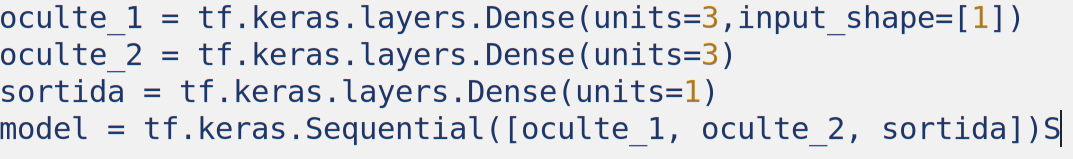
\includegraphics[width=0.5\textwidth]{./figures/3.png}
    \caption{Capes ocultes i la sortida d'una xarxa neuronal}
\end{figure}


Després de dissenyar l’estructura de la xarxa neuronal, cal ensenyar al model com aprendre i entrenar-se.
Per fer-ho utilitzem la variable \textbf{model}, a la qual ja havíem assignat les capes ocultes i la capa de sortida.
Tot seguit afegim la instrucció \textbf{.compile()}, que serveix per configurar el model abans de començar l’entrenament.

Dins de \texttt{.compile()} especifiquem el paràmetre \textbf{optimizer}, que indica la manera com el model ajustarà els pesos.
En aquest cas utilitzem \texttt{"adam"}, un optimitzador adaptatiu que redueix la velocitat d’aprenentatge quan detecta canvis bruscos en un pes,
l’augmenta quan el pes és estable i, alhora, recorda la direcció correcta per evitar oscil·lacions innecessàries.

A continuació, definim la funció de pèrdua amb el paràmetre \textbf{loss=\texttt{"mean\_squared\_error"}}.
La funció de pèrdua (\textit{loss}) mesura l’error del model i guia el procés d’aprenentatge.
En aquest cas, l’opció \texttt{mean squared error} (MSE, error quadràtic mitjà) és especialment útil en problemes de regressió,
ja que penalitza més fortament els errors grans i permet aconseguir prediccions més precises.


\begin{figure}[H]
    \centering
    
\includegraphics[width=0.5\textwidth]{./figures/5.png}
    \caption{Funció de pèrdua}
\end{figure}


\begin{figure}[H]
    \centering
    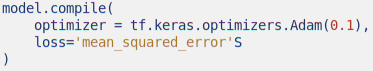
\includegraphics[width=0.5\textwidth]{./figures/4.png}
    \caption{Optimizació de la xarxa neuronal}
\end{figure}

Ara cal incloure la part crucial d'una xarxa neuronal: l'entrenament. Per fer-ho, utilitzem la variable \texttt{historial} per guardar l'evolució de l'entrenament i el model definit, \texttt{model}, aplicant-li el mètode \texttt{.fit()} que es el atribut que indica entrenament. Dins \texttt{.fit()} especifiquem, en ordre, les dades d'entrada (\texttt{celcius}), les dades de sortida (\texttt{fahrenheit}), el nombre de vegades que s'entrenarà la xarxa (\texttt{epochs=100}) i si volem mostrar el procés per pantalla (\texttt{verbose=1}, on 1 significa que sí i 0 que no).

A més, podem utilitzar \texttt{print()} per escriure comentaris o textos al terminal; en aquest cas hem posat \texttt{"Començem a entrenar..."} abans de començar i \texttt{"Model entrenat!"} un cop finalitzat l'entrenament.

\begin{figure}[H]
    \centering
    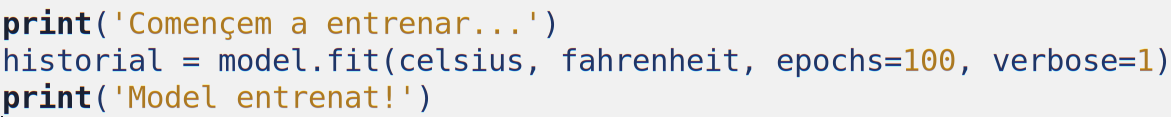
\includegraphics[width=0.5\textwidth]{./figures/6.png}
    \caption{L'entrenament de la xarxa neuronal}
\end{figure}

Després d’haver entrenat la xarxa neuronal i emmagatzemat l’evolució de la pèrdua a la variable \texttt{historial}, podem visualitzar com ha canviat la pèrdua a cada època utilitzant \texttt{matplotlib.pyplot}, una biblioteca de Python per crear gràfiques.

Primer, importem la biblioteca amb \texttt{import matplotlib.pyplot as plt}. A continuació, etiquetem els eixos de la gràfica amb \texttt{plt.xlabel("\# Època")} i \texttt{plt.ylabel("Magnitud de pèrdua")} per indicar què representa cada eix.

Per dibuixar la corba de la pèrdua utilitzem \texttt{plt.plot(historial.history[``loss''])}, que accedeix a la llista de valors de pèrdua que Keras ha guardat per cada època durant l’entrenament. Finalment, amb \texttt{plt.show()} mostrem la gràfica en una finestra del terminal o del notebook.

D’aquesta manera podem observar visualment si el model aprèn correctament, com disminueix la pèrdua al llarg de les èpoques i si hi ha comportaments irregulars que requeririen ajustar els paràmetres d’entrenament.

\begin{figure}[H]
    \centering
    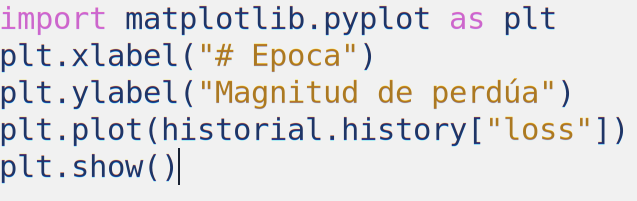
\includegraphics[width=0.5\textwidth]{./figures/7.png}
    \caption{La corba de pèrdua}
\end{figure}

Després d’haver entrenat la xarxa neuronal, podem fer prediccions amb nous valors d’entrada. Primer, utilitzem \texttt{print("Fem una predicció!")} per mostrar un missatge al terminal indicant que comença la predicció.

A continuació, fem servir \texttt{model.predict()} per calcular la predicció de la xarxa neuronal. En aquest cas, introduïm un valor de 100 graus Celsius amb \texttt{np.array([[100.0]], dtype=float)}, assegurant-nos que sigui un valor numèric decimal. El resultat s’emmagatzema a la variable \texttt{resultat}.

Finalment, utilitzem \texttt{print("El resultat es " + str(resultat) + " fahrenheit")} per mostrar la predicció obtinguda en Fahrenheit(el str es perque el variable resultat no sigui numeric sino un text). D’aquesta manera podem veure com el model converteix qualsevol temperatura de Celsius a Fahrenheit després de l’entrenament.


\begin{figure}[H]
    \centering
    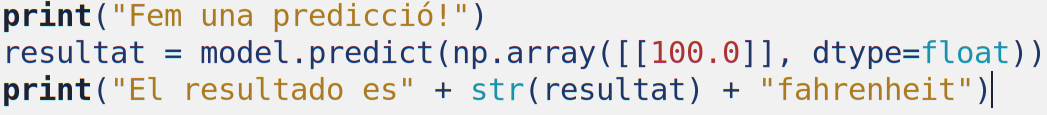
\includegraphics[width=0.5\textwidth]{./figures/8.png}
    \caption{Resultat de la predicció}
\end{figure}

Per a inspeccionar els pesos interns de la xarxa neuronal, podem utilitzar el mètode \texttt{.get\_weights()} en cada capa. Si el posem en els variables que haviem assignat les capes, per exemple, \texttt{oculte\_1.get\_weights()}, \texttt{oculte\_2.get\_weights()} i \texttt{sortida.get\_weights()} permeten veure els valors dels pesos i els biaixos que el model ha après durant l’entrenament, mostrant-los amb \texttt{print()}.


\begin{figure}[H]
    \centering
    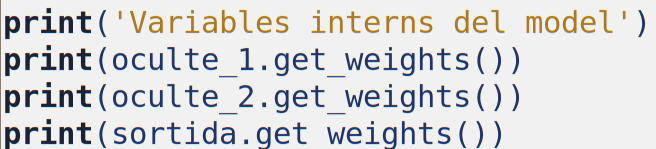
\includegraphics[width=0.5\textwidth]{./figures/9.png}
    \caption{Resultat de la predicció}
\end{figure}

Font: (\href{https://www.youtube.com/watch?v=iX_on3VxZzkhttps://www.youtube.com/watch?v=iX_on3VxZzk}{Xarxa neuronal amb Python})

\subsection{Predicció de les notes finals de matematiques }
Una vegada treballat amb la xarxa neuronal de celcius a fahrenheit, ja em trobo capacitat per fer la xarxa neuronal que ens haviem proposat, explicat en l'apartat \ref{sec:intr}




\section{Xarxa Neuronal amb fulls de calculs}\label{sec:11}
En aquest apartat continuarem amb la xarxa neuranal de regressió però aquesta vegada utilizarem un full de calculs per fer-ho.
L'estructura que utilitzarem per aquesta pràctica serà la del perceptró.

\begin{figure}[H]
    \centering
    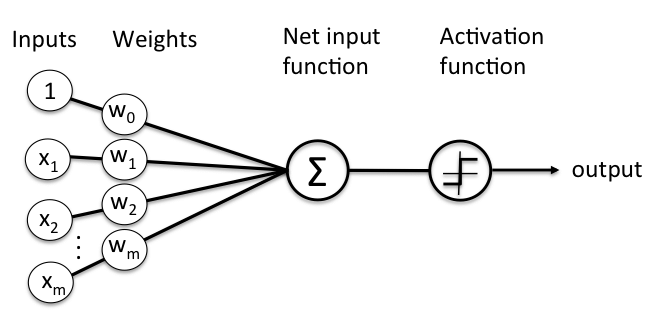
\includegraphics[width=0.5\textwidth]{./figures/perceptro.png}
    \caption{Estructura del perceptró}aaa
\end{figure}

Un cop sabem quina estructura utilitzarem, començarem la pràctica ordenant les dades de cada alumne del formulari en el full de càlculs

\begin{figure}[H]
    \centering
    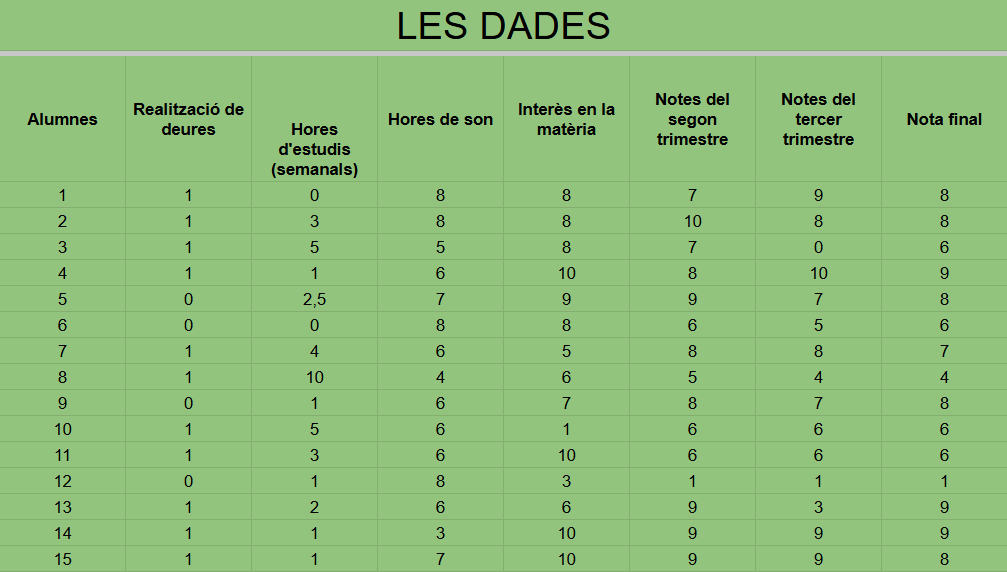
\includegraphics[width=0.5\textwidth]{./figures/Dades.png}
    \caption{Dades dels alumnes en el full de càlcul}
\end{figure}

Una vegada he ordenat tota la informació, he decidit representar els valors d'entrada d'una forma més senzilla d'entendre i curta, anomenantlos $xi$
\begin{itemize}
 \item \textbf Realització de deures: $x1$
 \item \textbf Hores d'estudis: $x2$
 \item \textbf Hores de son: $x3$
 \item \textbf Interès en la matèria: $x4$
 \item \textbf Notes del segon trimestre: $x5$
 \item \textbf Notes del tercer trimestre: $x6$
 \item \textbf Nota final: $y$
\end{itemize}

Aquestra representació queda així:

\begin{figure}[H]
    \centering
    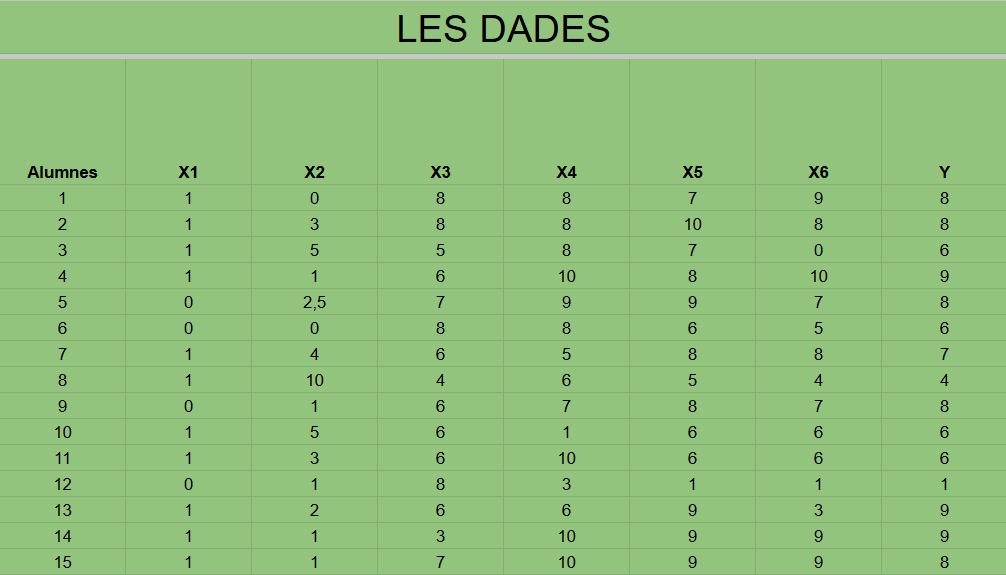
\includegraphics[width=0.5\textwidth]{./figures/Dades_resumides.png}
    \caption{Taula resumida}
\end{figure}

L'entrada de ``Realització de deures'' és una data binaria que nomès pot prendre valors 0 o 1.
\subsection{Normalització de dades}
Abans de continuar, és necessari explicar que és la normalització de dades.
La normalització de dades és una tècnica de procesament que consisteix en transformar dades de diferents escales a una escala comú, com per exemple del 0 al 1, aixó facilita la comparació i l'anàlisi de la xarxa neuronal i millora el seu rendiment. En el nostre cas, tenim dades binaries i dades ordinaries qe poden prendre qualsevol valor, aquest desequilibri afecta els càlculs posteriors si no es solucionen d'alguna manera.

Per aquesta raó, convertirem totes les dades en valors d'entre 0 i 1. Aquest procès implica calcular la miitjana de les dades i la desviació estàndar de cada variable. Per això utilitzant la fòrmula seguent:\\
$z = \frac{x - \mu}{\sigma}$\\

On:\\
$z$ És el valor normalitzat\\
$x$ És el valor original\\
$\mu$ És la mitjançan\\
$\sigma$ És la desviació estàndar\\

Aquests càlculs són fàcils d'obtenir amb les funcions que ens proporciona el full de càlcul.

\begin{figure}[H]
    \centering
    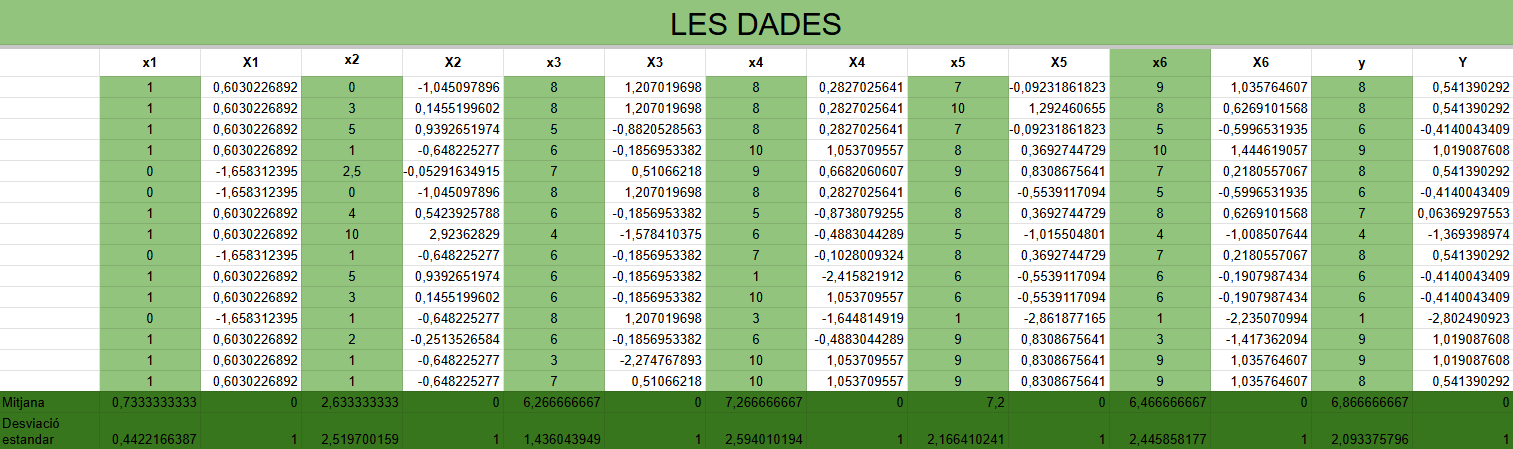
\includegraphics[width=0.5\textwidth]{./figures/Dades_normalitzades.png}
    \caption{Taula resumida}
\end{figure}

\subsection{Els pesos}
En una xarxa neuronal, cada valor d'entrada té el seu respectiu pes que determina la importància que té en la predicció final. AL començament de l'entrenament, assignarem a tots els pesos el mateix valor, ja que aquests es corregiran lentament durant el procès de l'entrenament.

\begin{figure}[H]
    \centering
    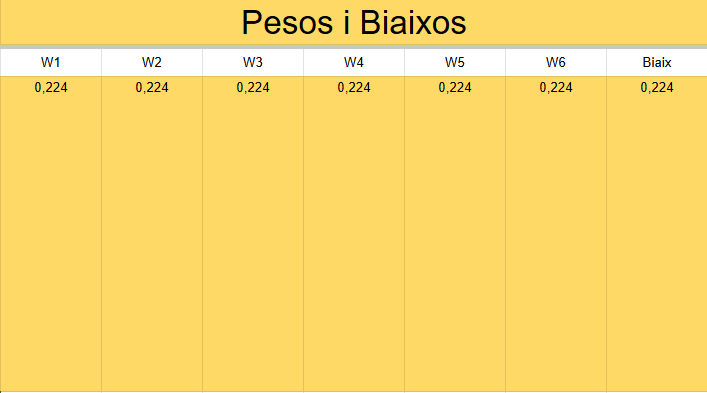
\includegraphics[width=0.5\textwidth]{./figures/Pesos.png}
    \caption{Taula dels pesos}
\end{figure}

Com es pot veure a la figura 6.9, he afegit 6 columnes pels pesos, respecte als 6 valors d'entrada, tambè he afegit una columna pel biaix, que serà la constant per millorar l'aust de les prediccions.

\subsection{Funció de pèrdua}
Ara que ja tenim les dades normalitzades i hem assignat els sues respectius pesos inicials, podrem aplicar la fòrmula de les xarxes neurnals artificials per calcular la predicció de les notes dels alumnes.
Recordem que la fòrmula de les xarxes neuronals artificials és:\\
\[
\sum w_i x_i + \text{biaix}
\]\\
Després d'aplicar aquesta fòrmula, obtindrem les prediccions de la nota final, tal com es mostra en la figura seguent.

\begin{figure}[H]
    \centering
    \includegraphics[width=0.5\textwidth]{./figures/Predicció.png}
    \caption{Prediccions del model}
\end{figure}

Cal recordar que aquest valors de la predicció són provisionals, ja que el valor dels pesos encara són imprecises.

El següent pas és entrenar el model per ajustar els pesos i fer més precís els valors de la predicció de la xarxa neuronal, per aconseguir-ho, utilitzarem un mètode d'optimització per ajustar els valors dels pesos, en aquest cas utilitzarem l'algoritme gradient descendent per minimitzar la funció d'error.

Per poder apicar aquest algoritme haurem d'afegir més columnes al nostre full de càlcul. Si restem els valors de la predicció ($Y$), amb els valors reals ($y$) obtindrem la diferència de la nota, es a dir, l'error del model.

\begin{figure}[H]
    \centering
    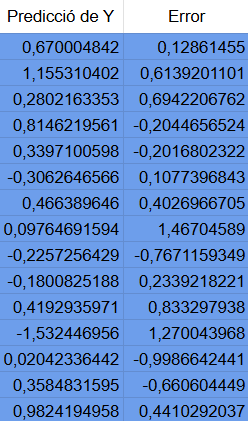
\includegraphics[width=0.5\textwidth]{./figures/Errors.png}
    \caption{Taula d'errors}
\end{figure}

Com podem veure en la figura 6.11, hem afegit 2 taules més, la taula d'error, on s'emmagatzema els errors del model, i la taula d'errors en positiu, aquesta última taula recull les dades de la taula d'error i agafa el valor absolut de les dades, fent que tots els valors es tornin positius, d'aquesta manera facilita els càlculs a l'hora de cambiar els paràmetres i s'aprecia la diferència de la predicció i el valor original.

Després d'aquest pas calcularem la mitjana de la taula dels errors en positius. El valor que dongui la mitjana ens ajudarà a saber si la xarxa està millorant la seva precisió, si aquest valor és petit, vol dir que l'error també és petit, fent el model més precís, en cada iteració hem d'aconseguir minimitzar aquest valor perquè el model sigui ho més precís possible.

\subsection{Canvis dels paràmetres}
Ara que ja sabem les funcions d'error de la primera predicció, ens toca entrenar el model per ajustar els pesos per disminuir els errors. Per dur aixó hem de tindre en compte ho següent: Com hem vist abans, l'error del model és la diferència que hi ha entre la predicció ($Y$) i el valor real ($y$), aixó vol dir que quan més gran sigui aquesta diferència, els pesos estaran més lluny del seu valor adequat, hem de trobar una forma per reduïr la diferència d'aquests valors.
Per altra banda, els valors d'entrada ($X$) es multipliquen pels seus respectius pesos ($W$), això vol dir que si el valor d'entrada ($X$) és petit, el seu pes ($W$) també serà petit, ja que aquests es multipliquen, com ho diu la fòrmula.
Per tant hem de tindre en compte dues coses: La diferència entre la predicció ($Y$) y el valor real ($y$) i el valor d'entrada ($X$) respecte a cada pes ($W$). Així que la fòrmula que utilitzarem per calcular els canvis de cada paràmetre serà:

\section{Comparació entre una xarxa neurnal creada per un llenguatge de programació netre una de fulls de calculs}

\section{Xarxa Neuronal amb un cas real}\label{sec:12}

%
\chapter{Resultats}
\label{c:Resultats}
\fbox{\emph{\textbf{\parbox{0.9\linewidth}{
Hem de tenir en compte de que les notes finals dels alumnes estan arrodonides, per tant considerarem que la predicció ha estat encertada si té un marge d'error menor a 0,5.}}}}
\section{Resultats de la xarxa neuronal en fulls de càlculs}
Desprès de finalitzar totes les etapes, els pesos s'han ajustat correctament i, encara que l'error no s'hagi pogut aproximar-se molt al zero absolut, ja és un valor molt petit que podem donar per bo. En la seguent figura podem veure els valors dels pesos finals del model.\\

\begin{figure}[H]
    \centering
    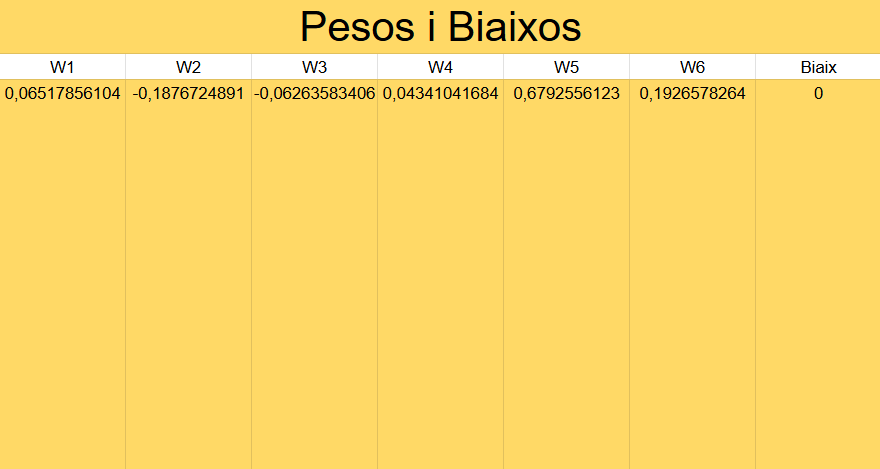
\includegraphics[width=0.5\textwidth]{./figures/Pesos_finals.png}
    \caption{Pesos finals del model}
\end{figure}

Amb aquests pesos, el model hauria de ser capaç d'obtenir unes prediccions precises respecte a la nota final dels alumnes, per obtenir els valors finals de la predicció, hem de convertir els valors normalitzats de la columna de la predicció de Y de l'última etapa en valors normals, aïllant en la mateixa fòrmula que vam emprar per normalitzar les dades.\\
$z = \frac{x - \mu}{\sigma}$\\

\begin{figure}[H]
    \centering
    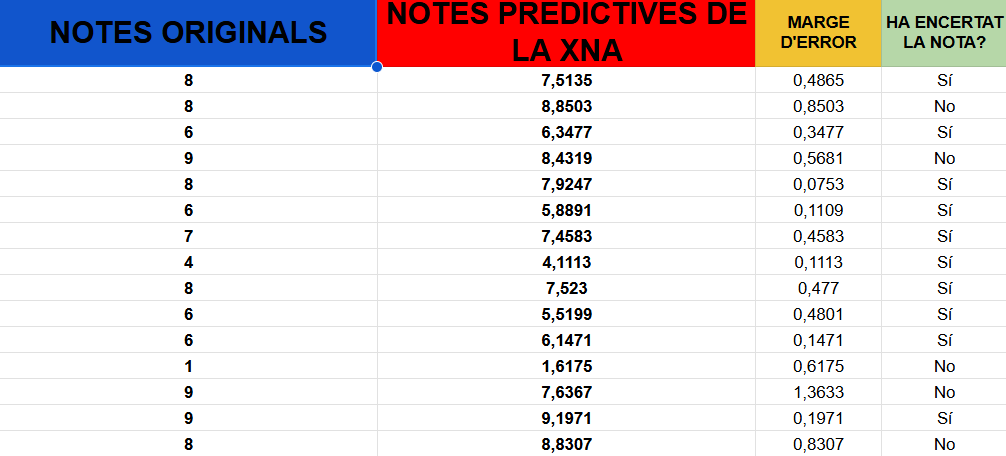
\includegraphics[width=0.5\textwidth]{./figures/Resultat_final.png}
    \caption{Prediccions finals de la pràctica}
\end{figure}

En la figura d'adalt, desprès de desnormalitzar els valors, he organitzat les notes inicials i les prediccions finals en unes taules per visualitzar-los millor, a un costat tenim les notes originals i per l'altre les predictives.
 Això ens dona que la xarxa neuronal ha encertat 10 notes de 15, per tant té una precisió aproximada del 66,7 percent.

\section{Comparació entre una xarxa neurnal creada per un llenguatge de programació netre una de fulls de calculs}
En aquest capítol, desprès de que cadascún de nosaltras haguèssim acabat les nostres respectives pràctiques, compararem els nostres resultats finals i veurem quina de les 2 formers és millor.

La principal diferencia que destaca entre aquest dues metodes de desenvolupament es la automització de l'aprenentatge (\textbf{Automatic machine}. En el cas dels fulls de càlcul, cal optimitzar i ajustar-ho tot manualment, cosa que esdevé un procés molt laboriós. En canvi, amb el llenguatge de programació, la XNA te'l fa tot el procés manual. Tanmateix, els fulls de calculs ho té tot més visual, permetent a l'usuari veure tot el treball, però en Python està oculta.
Per altre banda, en Python s'han utilitzat 18 enquestes y ha obtingut un resultat de 94,44\% de precisió, es a dir, ha encertat 17 notes de 18, per altre banda, el full de càlcul ha calgut de 15 enquestes y ha obtingut un 66,67\%, concretament ha encertat 10 de 15.
Podem observar que Python té una clara superioritat respecte als fulls de càlcul ja que té molta més precisió i ,a més, ha predit més notes. No obstant això, qualsevol persona que hagi fet una mica d'estadística pot manipular facilment un full de càcul, i hem de tenir en compte en que és molt més difícil fer la xarxa en Python perquè requereix de coneixements de programació.

En conclusió, si volguèssim una xarxa neuronal amb la màxima presició possible, Python seria una molt bona opció, però si no vols o no tens temps d'apendre un llenguatge de programació, és millor un full de càlcul, però s'ha de tenir en compte de que te molta menys precisió.























%

\chapter{Conclusions}

\label{c:conclusions}

Després dels resultats obtinguts, podem concloure que el treball està completat satisfactòriament. En aquest capítol presentem els assoliments dels objectius inicialment plantejats.

\begin{enumerate}

     \item \textbf{Entorn de treball professional:} S’ha aconseguit reproduir de manera notable el funcionament dels centres d’investigació en xarxes neuronals, amb l'ajuda de Linux, Git, GitHub i d'altres eines.

     \item \textbf{Escalabilitat:} La xarxa neuronal ha complert amb èxit aquest requisit, ja que és fàcilment ampliable mitjançant modificacions de paràmetres, incorporació de noves dades o augment de la seva complexitat.

     \item \textbf{Llibertat:} La publicació del projecte a GitHub ha permès convertir-lo en programari lliure, convertint-lo accessible, modificable i millorables per qualsevol persona.

     \item \textbf{Simplicitat i eficiència:} El model s’ha simplificat al màxim sense perdre eficàcia, assolint un equilibri entre senzillesa i rendiment.

     \item \textbf{Traçabilitat:} La publicació del projecte a GitHub dota al projecte de traçabilitat. El nostre repositori permet un seguiment pas per pas de l'elaboració del treball de recerca.

     \item \textbf{Xarxa neuronal:} En conclusió, tal com s’ha exposat en l’apartat comparatiu, la xarxa neuronal és superior al full de càlcul. Tanmateix, per a models simples continua sent recomanable l’ús del full de càlcul.

\end{enumerate}

Tot i que el treball ha estat dur i que ens ha calgut força esforç en alguns moments, l’experiència ha estat majoritàriament positiva. Hem gaudit molt en l’elaboració d’aquest projecte i hem tingut una gran motivació al llarg del procés. Gràcies a aquesta experiència hem pogut adquirir coneixements que mai ens havíem plantejat, cosa que ens permetrà tenir un cert avantatge en els inicis dels estudis universitaris. A més, aquest treball ens ha ajudat a millorar en la redacció, que fins ara havia estat un dels nostres punts febles.

\section{Recerca futura}
En el camp de la recerca, el final d'un treball pot ser l'inici d'un nou projecte de recerca. Per això creiem convenient fer propostes de com es podria continuar la nostra recerca.
% De cara al futur, hem definit una sèrie de possibles ampliacions que considerem beneficioses per a la nostra xarxa neuronal:


\begin{itemize}

\item Ampliar les sortides de la xarxa neuronal, ja que actualment només retorna un únic valor.

\item Millorar la velocitat de resposta, perquè en alguns casos el temps d’espera per obtenir un resultat precís era excessiu.

\item Desenvolupar nous models de la xarxa neuronal aplicats a casos reals, com el reconeixement de dígits, d’imatges o d’altres àmbits que hem considerat especialment interessants. Tanmateix, les limitacions en el temps i en l’extensió del treball no ens han permès dur-los a terme.

\item Crear una plataforma amb HTML\cite{HTML} i CSS\cite{CSS}, on publicar les noves actualitzacions i oferir guies a la comunitat per a principiants, tal com nosaltres ho érem en començar el TR.

\end{itemize}





\appendix
% \input{./capitols/rutinesLaTeX/rutinesLaTeX}
%
% \input{./capitols/codiJAVA/codiJAVA}
%
% \input{./capitols/bitacola/bitacola}


%---------------------------------------------------------------------
\chapter{{GNU Free Documentation License}}
\phantomsection  % so hyperref creates bookmarks
\addcontentsline{toc}{chapter}{GNU Free Documentation License}
%\label{label_fdl}

 \begin{center}

       Version 1.3, 3 November 2008


 Copyright \copyright{} 2000, 2001, 2002, 2007, 2008  Free Software Foundation, Inc.
 
 \bigskip
 
     \texttt{<https://fsf.org/>}
  
 \bigskip
 
 Everyone is permitted to copy and distribute verbatim copies
 of this license document, but changing it is not allowed.
\end{center}


\begin{center}
{\bf\large Preamble}
\end{center}

The purpose of this License is to make a manual, textbook, or other
functional and useful document ``free'' in the sense of freedom: to
assure everyone the effective freedom to copy and redistribute it,
with or without modifying it, either commercially or noncommercially.
Secondarily, this License preserves for the author and publisher a way
to get credit for their work, while not being considered responsible
for modifications made by others.

This License is a kind of ``copyleft'', which means that derivative
works of the document must themselves be free in the same sense.  It
complements the GNU General Public License, which is a copyleft
license designed for free software.

We have designed this License in order to use it for manuals for free
software, because free software needs free documentation: a free
program should come with manuals providing the same freedoms that the
software does.  But this License is not limited to software manuals;
it can be used for any textual work, regardless of subject matter or
whether it is published as a printed book.  We recommend this License
principally for works whose purpose is instruction or reference.


\begin{center}
{\Large\bf 1. APPLICABILITY AND DEFINITIONS\par}
\phantomsection
\addcontentsline{toc}{section}{1. APPLICABILITY AND DEFINITIONS}
\end{center}

This License applies to any manual or other work, in any medium, that
contains a notice placed by the copyright holder saying it can be
distributed under the terms of this License.  Such a notice grants a
world-wide, royalty-free license, unlimited in duration, to use that
work under the conditions stated herein.  The ``\textbf{Document}'', below,
refers to any such manual or work.  Any member of the public is a
licensee, and is addressed as ``\textbf{you}''.  You accept the license if you
copy, modify or distribute the work in a way requiring permission
under copyright law.

A ``\textbf{Modified Version}'' of the Document means any work containing the
Document or a portion of it, either copied verbatim, or with
modifications and/or translated into another language.

A ``\textbf{Secondary Section}'' is a named appendix or a front-matter section of
the Document that deals exclusively with the relationship of the
publishers or authors of the Document to the Document's overall subject
(or to related matters) and contains nothing that could fall directly
within that overall subject.  (Thus, if the Document is in part a
textbook of mathematics, a Secondary Section may not explain any
mathematics.)  The relationship could be a matter of historical
connection with the subject or with related matters, or of legal,
commercial, philosophical, ethical or political position regarding
them.

The ``\textbf{Invariant Sections}'' are certain Secondary Sections whose titles
are designated, as being those of Invariant Sections, in the notice
that says that the Document is released under this License.  If a
section does not fit the above definition of Secondary then it is not
allowed to be designated as Invariant.  The Document may contain zero
Invariant Sections.  If the Document does not identify any Invariant
Sections then there are none.

The ``\textbf{Cover Texts}'' are certain short passages of text that are listed,
as Front-Cover Texts or Back-Cover Texts, in the notice that says that
the Document is released under this License.  A Front-Cover Text may
be at most 5 words, and a Back-Cover Text may be at most 25 words.

A ``\textbf{Transparent}'' copy of the Document means a machine-readable copy,
represented in a format whose specification is available to the
general public, that is suitable for revising the document
straightforwardly with generic text editors or (for images composed of
pixels) generic paint programs or (for drawings) some widely available
drawing editor, and that is suitable for input to text formatters or
for automatic translation to a variety of formats suitable for input
to text formatters.  A copy made in an otherwise Transparent file
format whose markup, or absence of markup, has been arranged to thwart
or discourage subsequent modification by readers is not Transparent.
An image format is not Transparent if used for any substantial amount
of text.  A copy that is not ``Transparent'' is called ``\textbf{Opaque}''.

Examples of suitable formats for Transparent copies include plain
ASCII without markup, Texinfo input format, LaTeX input format, SGML
or XML using a publicly available DTD, and standard-conforming simple
HTML, PostScript or PDF designed for human modification.  Examples of
transparent image formats include PNG, XCF and JPG.  Opaque formats
include proprietary formats that can be read and edited only by
proprietary word processors, SGML or XML for which the DTD and/or
processing tools are not generally available, and the
machine-generated HTML, PostScript or PDF produced by some word
processors for output purposes only.

The ``\textbf{Title Page}'' means, for a printed book, the title page itself,
plus such following pages as are needed to hold, legibly, the material
this License requires to appear in the title page.  For works in
formats which do not have any title page as such, ``Title Page'' means
the text near the most prominent appearance of the work's title,
preceding the beginning of the body of the text.

The ``\textbf{publisher}'' means any person or entity that distributes
copies of the Document to the public.

A section ``\textbf{Entitled XYZ}'' means a named subunit of the Document whose
title either is precisely XYZ or contains XYZ in parentheses following
text that translates XYZ in another language.  (Here XYZ stands for a
specific section name mentioned below, such as ``\textbf{Acknowledgements}'',
``\textbf{Dedications}'', ``\textbf{Endorsements}'', or ``\textbf{History}''.)  
To ``\textbf{Preserve the Title}''
of such a section when you modify the Document means that it remains a
section ``Entitled XYZ'' according to this definition.

The Document may include Warranty Disclaimers next to the notice which
states that this License applies to the Document.  These Warranty
Disclaimers are considered to be included by reference in this
License, but only as regards disclaiming warranties: any other
implication that these Warranty Disclaimers may have is void and has
no effect on the meaning of this License.


\begin{center}
{\Large\bf 2. VERBATIM COPYING\par}
\phantomsection
\addcontentsline{toc}{section}{2. VERBATIM COPYING}
\end{center}

You may copy and distribute the Document in any medium, either
commercially or noncommercially, provided that this License, the
copyright notices, and the license notice saying this License applies
to the Document are reproduced in all copies, and that you add no other
conditions whatsoever to those of this License.  You may not use
technical measures to obstruct or control the reading or further
copying of the copies you make or distribute.  However, you may accept
compensation in exchange for copies.  If you distribute a large enough
number of copies you must also follow the conditions in section~3.

You may also lend copies, under the same conditions stated above, and
you may publicly display copies.


\begin{center}
{\Large\bf 3. COPYING IN QUANTITY\par}
\phantomsection
\addcontentsline{toc}{section}{3. COPYING IN QUANTITY}
\end{center}


If you publish printed copies (or copies in media that commonly have
printed covers) of the Document, numbering more than 100, and the
Document's license notice requires Cover Texts, you must enclose the
copies in covers that carry, clearly and legibly, all these Cover
Texts: Front-Cover Texts on the front cover, and Back-Cover Texts on
the back cover.  Both covers must also clearly and legibly identify
you as the publisher of these copies.  The front cover must present
the full title with all words of the title equally prominent and
visible.  You may add other material on the covers in addition.
Copying with changes limited to the covers, as long as they preserve
the title of the Document and satisfy these conditions, can be treated
as verbatim copying in other respects.

If the required texts for either cover are too voluminous to fit
legibly, you should put the first ones listed (as many as fit
reasonably) on the actual cover, and continue the rest onto adjacent
pages.

If you publish or distribute Opaque copies of the Document numbering
more than 100, you must either include a machine-readable Transparent
copy along with each Opaque copy, or state in or with each Opaque copy
a computer-network location from which the general network-using
public has access to download using public-standard network protocols
a complete Transparent copy of the Document, free of added material.
If you use the latter option, you must take reasonably prudent steps,
when you begin distribution of Opaque copies in quantity, to ensure
that this Transparent copy will remain thus accessible at the stated
location until at least one year after the last time you distribute an
Opaque copy (directly or through your agents or retailers) of that
edition to the public.

It is requested, but not required, that you contact the authors of the
Document well before redistributing any large number of copies, to give
them a chance to provide you with an updated version of the Document.

\clearpage
\begin{center}
{\Large\bf 4. MODIFICATIONS\par}
\phantomsection
\addcontentsline{toc}{section}{4. MODIFICATIONS}
\end{center}

You may copy and distribute a Modified Version of the Document under
the conditions of sections 2 and 3 above, provided that you release
the Modified Version under precisely this License, with the Modified
Version filling the role of the Document, thus licensing distribution
and modification of the Modified Version to whoever possesses a copy
of it.  In addition, you must do these things in the Modified Version:

\begin{itemize}
\item[A.] 
   Use in the Title Page (and on the covers, if any) a title distinct
   from that of the Document, and from those of previous versions
   (which should, if there were any, be listed in the History section
   of the Document).  You may use the same title as a previous version
   if the original publisher of that version gives permission.
   
\item[B.]
   List on the Title Page, as authors, one or more persons or entities
   responsible for authorship of the modifications in the Modified
   Version, together with at least five of the principal authors of the
   Document (all of its principal authors, if it has fewer than five),
   unless they release you from this requirement.
   
\item[C.]
   State on the Title page the name of the publisher of the
   Modified Version, as the publisher.
   
\item[D.]
   Preserve all the copyright notices of the Document.
   
\item[E.]
   Add an appropriate copyright notice for your modifications
   adjacent to the other copyright notices.
   
\item[F.]
   Include, immediately after the copyright notices, a license notice
   giving the public permission to use the Modified Version under the
   terms of this License, in the form shown in the Addendum below.
   
\item[G.]
   Preserve in that license notice the full lists of Invariant Sections
   and required Cover Texts given in the Document's license notice.
   
\item[H.]
   Include an unaltered copy of this License.
   
\item[I.]
   Preserve the section Entitled ``History'', Preserve its Title, and add
   to it an item stating at least the title, year, new authors, and
   publisher of the Modified Version as given on the Title Page.  If
   there is no section Entitled ``History'' in the Document, create one
   stating the title, year, authors, and publisher of the Document as
   given on its Title Page, then add an item describing the Modified
   Version as stated in the previous sentence.
   
\item[J.]
   Preserve the network location, if any, given in the Document for
   public access to a Transparent copy of the Document, and likewise
   the network locations given in the Document for previous versions
   it was based on.  These may be placed in the ``History'' section.
   You may omit a network location for a work that was published at
   least four years before the Document itself, or if the original
   publisher of the version it refers to gives permission.
   
\item[K.]
   For any section Entitled ``Acknowledgements'' or ``Dedications'',
   Preserve the Title of the section, and preserve in the section all
   the substance and tone of each of the contributor acknowledgements
   and/or dedications given therein.
   
\item[L.]
   Preserve all the Invariant Sections of the Document,
   unaltered in their text and in their titles.  Section numbers
   or the equivalent are not considered part of the section titles.
   
\item[M.]
   Delete any section Entitled ``Endorsements''.  Such a section
   may not be included in the Modified Version.
   
\item[N.]
   Do not retitle any existing section to be Entitled ``Endorsements''
   or to conflict in title with any Invariant Section.
   
\item[O.]
   Preserve any Warranty Disclaimers.
\end{itemize}

If the Modified Version includes new front-matter sections or
appendices that qualify as Secondary Sections and contain no material
copied from the Document, you may at your option designate some or all
of these sections as invariant.  To do this, add their titles to the
list of Invariant Sections in the Modified Version's license notice.
These titles must be distinct from any other section titles.

You may add a section Entitled ``Endorsements'', provided it contains
nothing but endorsements of your Modified Version by various
parties---for example, statements of peer review or that the text has
been approved by an organization as the authoritative definition of a
standard.

You may add a passage of up to five words as a Front-Cover Text, and a
passage of up to 25 words as a Back-Cover Text, to the end of the list
of Cover Texts in the Modified Version.  Only one passage of
Front-Cover Text and one of Back-Cover Text may be added by (or
through arrangements made by) any one entity.  If the Document already
includes a cover text for the same cover, previously added by you or
by arrangement made by the same entity you are acting on behalf of,
you may not add another; but you may replace the old one, on explicit
permission from the previous publisher that added the old one.

The author(s) and publisher(s) of the Document do not by this License
give permission to use their names for publicity for or to assert or
imply endorsement of any Modified Version.


\begin{center}
{\Large\bf 5. COMBINING DOCUMENTS\par}
\phantomsection
\addcontentsline{toc}{section}{5. COMBINING DOCUMENTS}
\end{center}


You may combine the Document with other documents released under this
License, under the terms defined in section~4 above for modified
versions, provided that you include in the combination all of the
Invariant Sections of all of the original documents, unmodified, and
list them all as Invariant Sections of your combined work in its
license notice, and that you preserve all their Warranty Disclaimers.

The combined work need only contain one copy of this License, and
multiple identical Invariant Sections may be replaced with a single
copy.  If there are multiple Invariant Sections with the same name but
different contents, make the title of each such section unique by
adding at the end of it, in parentheses, the name of the original
author or publisher of that section if known, or else a unique number.
Make the same adjustment to the section titles in the list of
Invariant Sections in the license notice of the combined work.

In the combination, you must combine any sections Entitled ``History''
in the various original documents, forming one section Entitled
``History''; likewise combine any sections Entitled ``Acknowledgements'',
and any sections Entitled ``Dedications''.  You must delete all sections
Entitled ``Endorsements''.

\clearpage
\begin{center}
{\Large\bf 6. COLLECTIONS OF DOCUMENTS\par}
\phantomsection
\addcontentsline{toc}{section}{6. COLLECTIONS OF DOCUMENTS}
\end{center}

You may make a collection consisting of the Document and other documents
released under this License, and replace the individual copies of this
License in the various documents with a single copy that is included in
the collection, provided that you follow the rules of this License for
verbatim copying of each of the documents in all other respects.

You may extract a single document from such a collection, and distribute
it individually under this License, provided you insert a copy of this
License into the extracted document, and follow this License in all
other respects regarding verbatim copying of that document.


\begin{center}
{\Large\bf 7. AGGREGATION WITH INDEPENDENT WORKS\par}
\phantomsection
\addcontentsline{toc}{section}{7. AGGREGATION WITH INDEPENDENT WORKS}
\end{center}


A compilation of the Document or its derivatives with other separate
and independent documents or works, in or on a volume of a storage or
distribution medium, is called an ``aggregate'' if the copyright
resulting from the compilation is not used to limit the legal rights
of the compilation's users beyond what the individual works permit.
When the Document is included in an aggregate, this License does not
apply to the other works in the aggregate which are not themselves
derivative works of the Document.

If the Cover Text requirement of section~3 is applicable to these
copies of the Document, then if the Document is less than one half of
the entire aggregate, the Document's Cover Texts may be placed on
covers that bracket the Document within the aggregate, or the
electronic equivalent of covers if the Document is in electronic form.
Otherwise they must appear on printed covers that bracket the whole
aggregate.


\begin{center}
{\Large\bf 8. TRANSLATION\par}
\phantomsection
\addcontentsline{toc}{section}{8. TRANSLATION}
\end{center}


Translation is considered a kind of modification, so you may
distribute translations of the Document under the terms of section~4.
Replacing Invariant Sections with translations requires special
permission from their copyright holders, but you may include
translations of some or all Invariant Sections in addition to the
original versions of these Invariant Sections.  You may include a
translation of this License, and all the license notices in the
Document, and any Warranty Disclaimers, provided that you also include
the original English version of this License and the original versions
of those notices and disclaimers.  In case of a disagreement between
the translation and the original version of this License or a notice
or disclaimer, the original version will prevail.

If a section in the Document is Entitled ``Acknowledgements'',
``Dedications'', or ``History'', the requirement (section~4) to Preserve
its Title (section~1) will typically require changing the actual
title.


\begin{center}
{\Large\bf 9. TERMINATION\par}
\phantomsection
\addcontentsline{toc}{section}{9. TERMINATION}
\end{center}


You may not copy, modify, sublicense, or distribute the Document
except as expressly provided under this License.  Any attempt
otherwise to copy, modify, sublicense, or distribute it is void, and
will automatically terminate your rights under this License.

However, if you cease all violation of this License, then your license
from a particular copyright holder is reinstated (a) provisionally,
unless and until the copyright holder explicitly and finally
terminates your license, and (b) permanently, if the copyright holder
fails to notify you of the violation by some reasonable means prior to
60 days after the cessation.

Moreover, your license from a particular copyright holder is
reinstated permanently if the copyright holder notifies you of the
violation by some reasonable means, this is the first time you have
received notice of violation of this License (for any work) from that
copyright holder, and you cure the violation prior to 30 days after
your receipt of the notice.

Termination of your rights under this section does not terminate the
licenses of parties who have received copies or rights from you under
this License.  If your rights have been terminated and not permanently
reinstated, receipt of a copy of some or all of the same material does
not give you any rights to use it.


\begin{center}
{\Large\bf 10. FUTURE REVISIONS OF THIS LICENSE\par}
\phantomsection
\addcontentsline{toc}{section}{10. FUTURE REVISIONS OF THIS LICENSE}
\end{center}


The Free Software Foundation may publish new, revised versions
of the GNU Free Documentation License from time to time.  Such new
versions will be similar in spirit to the present version, but may
differ in detail to address new problems or concerns.  See
\texttt{https://www.gnu.org/licenses/}.

Each version of the License is given a distinguishing version number.
If the Document specifies that a particular numbered version of this
License ``or any later version'' applies to it, you have the option of
following the terms and conditions either of that specified version or
of any later version that has been published (not as a draft) by the
Free Software Foundation.  If the Document does not specify a version
number of this License, you may choose any version ever published (not
as a draft) by the Free Software Foundation.  If the Document
specifies that a proxy can decide which future versions of this
License can be used, that proxy's public statement of acceptance of a
version permanently authorizes you to choose that version for the
Document.


\begin{center}
{\Large\bf 11. RELICENSING\par}
\phantomsection
\addcontentsline{toc}{section}{11. RELICENSING}
\end{center}


``Massive Multiauthor Collaboration Site'' (or ``MMC Site'') means any
World Wide Web server that publishes copyrightable works and also
provides prominent facilities for anybody to edit those works.  A
public wiki that anybody can edit is an example of such a server.  A
``Massive Multiauthor Collaboration'' (or ``MMC'') contained in the
site means any set of copyrightable works thus published on the MMC
site.

``CC-BY-SA'' means the Creative Commons Attribution-Share Alike 3.0
license published by Creative Commons Corporation, a not-for-profit
corporation with a principal place of business in San Francisco,
California, as well as future copyleft versions of that license
published by that same organization.

``Incorporate'' means to publish or republish a Document, in whole or
in part, as part of another Document.

An MMC is ``eligible for relicensing'' if it is licensed under this
License, and if all works that were first published under this License
somewhere other than this MMC, and subsequently incorporated in whole
or in part into the MMC, (1) had no cover texts or invariant sections,
and (2) were thus incorporated prior to November 1, 2008.

The operator of an MMC Site may republish an MMC contained in the site
under CC-BY-SA on the same site at any time before August 1, 2009,
provided the MMC is eligible for relicensing.

\clearpage
\begin{center}
{\Large\bf ADDENDUM: How to use this License for your documents\par}
\phantomsection
\addcontentsline{toc}{section}{ADDENDUM: How to use this License for your documents}
\end{center}

To use this License in a document you have written, include a copy of
the License in the document and put the following copyright and
license notices just after the title page:

\bigskip
\begin{quote}
    Copyright \copyright{}  YEAR  YOUR NAME.
    Permission is granted to copy, distribute and/or modify this document
    under the terms of the GNU Free Documentation License, Version 1.3
    or any later version published by the Free Software Foundation;
    with no Invariant Sections, no Front-Cover Texts, and no Back-Cover Texts.
    A copy of the license is included in the section entitled ``GNU
    Free Documentation License''.
\end{quote}
\bigskip
    
If you have Invariant Sections, Front-Cover Texts and Back-Cover Texts,
replace the ``with \dots\ Texts.''\ line with this:

\bigskip
\begin{quote}
    with the Invariant Sections being LIST THEIR TITLES, with the
    Front-Cover Texts being LIST, and with the Back-Cover Texts being LIST.
\end{quote}
\bigskip
    
If you have Invariant Sections without Cover Texts, or some other
combination of the three, merge those two alternatives to suit the
situation.

If your document contains nontrivial examples of program code, we
recommend releasing these examples in parallel under your choice of
free software license, such as the GNU General Public License,
to permit their use in free software.

%---------------------------------------------------------------------


\renewcommand\bibname{Bibliografia}
\bibliographystyle{./bibliografia/caplain}
\bibliography{./bibliografia/myBiblio}
\addcontentsline{toc}{chapter}{Bibliografia}
\label{b:bibliography}

% \listoffigures
% \listoftables




\end{document} 
